\documentclass{article}

\usepackage{amsmath}
\usepackage{txfonts}
\usepackage{graphicx}
\usepackage{booktabs}
\usepackage{url}
\usepackage{natbib}
\usepackage{rotating}
\usepackage{adjustbox}
\graphicspath{{figures/}}
\bibliographystyle{biblio.bst}

\title{Probabilistic Forecasting of Geomagnetic Indices using Gaussian Process Models}

\begin{document}


\begin{abstract}

In this chapter, we give the reader an in depth view into building of probabilistic forecasting models for geomagnetic time series using the \emph{Gaussian Process} methodology outlined in the previous chapters. We highlight design decisions and practical issues that must be addressed in order to use \emph{Gaussian Process} models for probabilistic prediction of a quantity of interest. As a pedagogical example, we formulate, train and test a family of \emph{Gaussian Process} Auto-Regressive models for one hour ahead prediction of the $Dst$ geomagnetic index.  

\end{abstract}

\section{Geomagnetic Time Series \& Forecasting}

The Earth's magnetosphere is the region above the ionosphere that is defined by the extent of the Earth's magnetic field in space. It extends several tens of thousands of kilometers into space, a region which is impinged upon constantly by the solar wind. Ionized plasma ejected by the sun couples with the Earth's magnetic field in a complex manner leading to highly non-linear and chaotic processes which determine the state of the magnetosphere. It is quite common to reduce these complex dependencies by condensing the state of the Earth's magnetosphere into a set of geomagnetic indices.

Geomagnetic indices come in various forms, they may take continuous or discrete values and may be defined with varying time resolutions. Their values are often calculated by averaging or combining a number of readings taken by instruments, usually magnetometers, around the Earth. Each geomagnetic index is a proxy for a particular kind of phenomenon. Some common indices are the $Kp$, $Dst$ and the $AE$ index.

\begin{enumerate}
    \item $Kp$: The Kp-index is a discrete valued global geomagnetic
      activity index and is based on 3 hour measurements of the
      K-indices \citep{Bartels}. The K-index itself is a three hour
      long quasi-logarithmic local index of the geomagnetic activity,
      relative to a quiet day curve for the given location.
    
    \item $AE$: The Auroral Electrojet Index, $AE$, is designed to
      provide a global, quantitative measure of auroral zone magnetic
      activity produced by enhanced ionospheric currents flowing below
      and within the auroral oval \citep{AEIndex}. It is a continuous index which is calculated every hour.
    
    \item $Dst$: A continuous hourly index which measures the
      magnitude of the magnetic field induced by near equatorial ring
      currents \citep{DesslerAndParker}. A large negative value of
      $Dst$ ($ \leq -100 \ nT$) indicates occurrence of geomagnetic
      storm events which are of particular importance in space weather
      prediction due to their adverse effects on telecommunications
      infrastructure, navigation systems, power grids, satellites etc. 
\end{enumerate}

Space weather forecasting systems usually use in-situ measurements of
solar wind parameters, taken by satellites, as well as historical data
of indices to produce forecasts for various geomagnetic time
series. Real time data of solar wind parameters are recorded by the \emph{ACE}
and \emph{DISCOVR} missions. Geomagnetic indices are often recorded in
ground based measurements. The the \emph{Space Physics Data Facility}
(SPDF) hosted by NASA is a gateway for accessing data from a variety
of sources, including those mentioned above.

\section{Data Source: OMNI}
The \emph{OMNI} data set is a collation of in-situ measurements taken by orbiting satellites and ground based measurements of geomagnetic indices. The data itself is represented as time averaged versions of the various quantities and is available at two frequencies, by hour and by minute. The quantities recorded can be broadly classified into two groups.

\begin{enumerate}

  \item Plasma Parameters and Magnetic fields: Measurements of the solar wind particularly the solar wind speed, flow angles, pressure, proton temperature, proton density and field measurements such as strength of electric and magnetic fields as well as their components in various geomagnetic coordinate systems.
  
  \item Indices: $Kp$, $Ae$, $Ap$, $Dst$, sunspot number.
  
\end{enumerate}

To get a more indepth understanding about the \emph{OMNI} data, interested readers are encouraged to visit the NASA omni web service (\url{https://omniweb.gsfc.nasa.gov}).

In this chapter for the purpose of exposition, we will focus on one hour ahead prediction of the $Dst$ time series. From the data we will use time histories of $Dst$, solar wind speed $V$ and the $z$-component of the interplanetary magnetic field $B_z$. Our choice is motivated by both physical and practical considerations: solar wind speed and interplanetary magnetic field are important external drivers for particle injection into the magnetosphere and they have large coverage in the \emph{OMNI} data with relatively lesser number of missing records.

\section{$Dst$ Forecasting}

\subsection{State of the art}

A number of modeling techniques have been applied for the prediction of the $Dst$ index. One of the earliest forecasting techniques involves calculating the $Dst(t)$ as a solution of an \emph{Ordinary Differential Equation} (ODE) which expressed the rate of change of $Dst(t)$ as a combination of two terms: decay and injection $\frac{d Dst(t)}{dt} = Q(t) - \frac{Dst(t)}{\tau}$, where $Q(t)$ relates to the particle injection from the plasma sheet into the inner magnetosphere. This method was presented first by \citet{JGR:JGR10260} and later modified and extended in works such as \citet{Wang:Dst}, \citet{JGRA:JGRA14856}, \citet{Ballatore2014} and others.

%Talk about NARMAX Dst
Important empirical geomagnetic prediction models include the \emph{Nonlinear Auto-Regessive Moving Average with eXogenous inputs} (NARMAX) methodology (see \citet{doi:10.1080/00207178908559767}, \citet{GRL:GRL13494}, \citet{GRL:GRL20944}, \citet{JGRA:JGRA18657}, \citet{balikhin:narmax}, \citet{JGRA:JGRA20661}, \citet{JGRA:JGRA50192}) and \emph{Artificial Neural Networks} (ANN) based models (\citet{Lund}, \citet{JGRA:JGRA17461}, \citet{SWE:SWE286}, \citet{pallocchia:hal-00318011}) for time series prediction of $Dst$ and $Kp$ indices from interplanetary magnetic field data and solar wind parameters. 

\subsection{Probabilistic Forecasting}
%Talk about need for probabilistic forecasts.ny
Although much research has been done on prediction of the $Dst$ index, much less has been done on probabilistic forecasting of $Dst$. One such work described in \citet{McPherron:2013} involves identification of high speed solar wind streams using the WSA model, using predictions of high speed streams to construct ensembles of $Dst$ trajectories which yield the quartiles of $Dst$ time series. 

Probabilistic forecasting is of particular importance in geophysics applications as the end users of forecasts often require confidence bounds on the said forecasts. It is in this context where \emph{Gaussian Processes} become especially attractive due to their inherent probabilistic formulation and tractability of exact inference.


\section{Gaussian Processes}

\emph{Gaussian Processes} first appeared in machine learning research in \citet{Neal:1996:BLN:525544}, as the limiting case of Bayesian inference performed on neural networks with infinitely many neurons in the hidden layers. Although their inception in the machine learning community is recent, their origins can be traced back to the geo-statistics research community where they are known as \emph{Kriging} methods \citep{krige1951statistical}. In pure Mathematics, \emph{Gaussian Processes} have been studied extensively and their existence was first proven by Kolmogorov's extension theorem \citep{tao2011introduction}. The reader is referred to \citet{Rasmussen:2005:GPM:1162254} for an in depth treatment of Gaussian Processes in machine learning.

Without going into too many details, we give a quick recap of the formulation and exact inference in \emph{Gaussian Process Regression} (GPR) models. 

\subsection{Gaussian Process Regression: Formulation}

Our aim is to infer an unknown function $f(\mathbf{x})$ from its noise corrupted measurements $(\mathbf{x}_i, y_i)$ where $y_i = f(\mathbf{x}_i) + \epsilon$ and $\epsilon \sim \mathcal{N}(0, \sigma^2)$ is independent and identically distributed Gaussian noise.

A \emph{Gaussian Process} model represents the finite dimensional probability distribution of $f(\mathbf{x}_i)$ by a multivariate gaussian having a particular structure for its mean and covariance as shown in \ref{eq:normal} - \ref{eq:sto}.

\begin{align}
 \mathbf{f} = & \left( \begin{array}{c} f(\mathbf{x}_1) \\ f(\mathbf{x}_2) \\ \vdots \\ f(\mathbf{x}_N) \end{array} \right) \label{eq:fvalues}\\
 \vspace{2\baselineskip}
 \mathbf{f} | \mathbf{x}_1, \cdots, \mathbf{x}_N \sim & \mathcal{N}\left( \mathbf{m}, \mathbf{K} \right)  \label{eq:normal}\\
 \vspace{2\baselineskip}
 \mathbb{P}( \mathbf{f} \ | \ \mathbf{x}_1, \cdots, \mathbf{x}_N) = & \frac{1}{(2\pi)^{n/2} det(\mathbf{K})^{1/2}} exp \left(-\frac{1}{2} (\mathbf{f} - \mathbf{m})^T \mathbf{K}^{-1} (\mathbf{f} - \mathbf{m}) \right) \label{eq:sto}
\end{align}

In order to uniquely define the distribution of $\mathbf{f}$, it is
required to specify the mean $\mathbf{m}$ and the covariance matrix
$\mathbf{K}$. For this probability density to be valid, there are further requirements imposed on $\mathbf{K}$: 

\begin{enumerate}
      \item Symmetry: $\mathbf{K}_{ij} = \mathbf{K}_{ji} \ \forall i,j \in {1, \cdots, N} $ 
      \item Positive Semi-definiteness: $\mathbf{z}^T \mathbf{K} \mathbf{z} \geq 0 \ \forall \mathbf{z} \in \mathbb{R}^N$  
\end{enumerate}

In \emph{Gaussian Processes} the individual elements of $\mathbf{x}$ and $\mathbf{K}$ are specified in the form of functions as shown below.

\begin{align}
      \mu_i = & \mathbb{E}[f(\mathbf{x}_i)] := m(\mathbf{x}_i) \\
      \Lambda_{ij} = & \mathbb{E}[(f(\mathbf{x}_i) - \mu_i)(f(\mathbf{x}_j) - \mu_j)] := K(\mathbf{x}_i, \mathbf{x}_j)
\end{align}

In the machine learning community, $m(.)$ and $K(.,.)$ are known as the \emph{mean function} and \emph{covariance function} or \emph{kernel function} of the process respectively. Giving a closed form expression for $m(.)$ and $K(.,.)$ uniquely specifies a particular \emph{Gaussian Process} and so a GP model is often expressed in the following notation.

\begin{equation}
    f(\mathbf{x}) \sim \mathcal{GP}(m(\mathbf{x}), K(\mathbf{x}, \mathbf{x}'))
\end{equation}

\subsection{Gaussian Process Regression: Inference}

In order to generate predictions $f(\mathbf{x}^{*}_i)$ for a set of test points $ {\mathbf{x}^{*}_i : \forall i \in 1, \cdots, M} $. Using the multivariate Gaussian distribution in equation (\ref{eq:sto}) we can construct the joint distribution of $f(\mathbf{x})$ over the training and test points.

\begin{align}
    \mathbf{f}_* = & \left( \begin{array}{c} f(\mathbf{x^{*}_1}) \\ f(\mathbf{x^{*}_2}) \\ \vdots \\ f(\mathbf{x^{*}_M}) \end{array} \right)_{M \times 1} \\
     \vspace{4\baselineskip}
    \left( \begin{array}{c} \mathbf{y} \\ \mathbf{f_*} \end{array} \right) | \ \ \mathbf{X}, \mathbf{X}_* \sim & 
    \mathcal{N}\left(\mathbf{0}, \left[ \begin{array}{cc} \mathbf{K} + \sigma^{2} \mathbf{I} & \mathbf{K}_{*} \\ \mathbf{K}_{*}^T & \mathbf{K}_{**} \end{array} \right ] \right) \label{eq:dist}
\end{align}

Probabilistic predictions $f_*$ can be generated by constructing the conditional distribution $\mathbf{f_*}|\mathbf{X},\mathbf{y},\mathbf{X_*}$ which is also a multivariate gaussian as shown in equation \ref{eq:posterior}.

\begin{align}
    & \mathbf{f_*}|\mathbf{X},\mathbf{y},\mathbf{X_*} \sim \mathcal{N}(\mathbf{\bar{f}_*}, \Sigma_*)  \label{eq:posterior} \\
    & \mathbf{\bar{f}_*} =  \ \mathbf{K}^T_{*} [\mathbf{K} + \sigma^{2} \mathbf{I}]^{-1} \mathbf{y} \label{eq:posteriormean} \\
    & \Sigma_* = \ \mathbf{K}_{**} - \mathbf{K}^T_{*} \left(\mathbf{K} + \sigma^{2} \mathbf{I}\right)^{-1} \mathbf{K}_{*} \label{eq:posteriorcov}
\end{align}

\section{One Hour Ahead $Dst$ Prediction: Formulation} \label{sec:osa}

Below in equations (\ref{eq:Dst}) - (\ref{eq:DstGP}) we outline a \emph{Gaussian Process} formulation for \emph{OSA} prediction of $Dst$. A vector of features $\mathbf{x}_{t-1}$ is used as input to an unknown function $f(\mathbf{x}_{t-1})$.

The features $\mathbf{x}_{t-1}$ can be any collection of quantities in the hourly resolution OMNI data set. Generally $\mathbf{x}_{t-1}$ are time histories of $Dst$ and other important variables such as plasma pressure $p(t)$, solar wind speed $V(t)$, $z$ component of the interplanetary magnetic field $B_z(t)$.


\begin{align}
    Dst(t) & =  f(\mathbf{x}_{t-1}) + \epsilon \label{eq:Dst} \\
    \epsilon & \sim  \mathcal{N}(0, \sigma^2) \label{eq:GPNoise} \\
    f(x_t) & \sim  \mathcal{GP}(m(\mathbf{x}_t), K_{osa}(\mathbf{x}_t, \mathbf{x}_s)) \label{eq:DstGP} \\
\end{align}

We consider two choices for the input features $\mathbf{x}_{t-1}$ leading to two variants of \emph{Gaussian Process} regression for $Dst$ time series prediction.

\subsection{Gaussian Process Auto-Regressive (GP-AR)} \label{sec:gpar}

The simplest auto-regressive models for \emph{OSA} prediction of $Dst$ are those that use only the history of $Dst$ to construct input features for model training. The input features $\mathbf{x}_{t-1}$ at each time step are the history of $Dst(t)$ until a time lag of $p$ hours.

\begin{align*}
    \mathbf{x}_{t-1} = & \left(Dst(t-1), \cdots , Dst(t-p+1)\right)
\end{align*}

\subsection{Gaussian Process Auto-Regressive with eXogenous inputs (GP-ARX)} \label{sec:gparx}

Auto-regressive models can be augmented by including exogenous quantities in the inputs $\mathbf{x}_{t-1}$ at each time step, in order to improve predictive accuracy. $Dst$ gives a measure of ring currents, which are modulated by plasma sheet particle injections into the inner magnetosphere during substorms. Studies have shown that the substorm occurrence rate increases with solar wind velocity (high speed streams) \citet{Kissinger2011,Newell2016}. Prolonged southward interplanetary magnetic field (IMF) $z$-component ($B_z$) is needed for sub-storms to occur \citet{McPherron1986}. An increase in the solar wind electric field, $V_{sw}B_z$, can increase the dawn-dusk electric field in the magnetotail, which in turn determines the amount of plasma sheet particle that move to the inner magnetosphere \citet{Friedel2001}. Therefore, our exogenous parameters consist of solar wind velocity $V_{sw}$ and IMF $B_z$.   

In this model we choose distinct time lags $p$, $p_{v}$ and $p_{b}$ for $Dst$, $V$ and $B_z$ respectively.
    
\begin{align*}
       \mathbf{x}_{t-1} & = (Dst(t-1), \cdots , Dst(t-p+1), \\
        & \ \ \ \ \  V_{sw}(t-1), \cdots, V_{sw}(t-p_{v}+1),\\
        & \ \ \ \ \  B_{z}(t-1), \cdots, B_{z}(t-p_{b}+1))
\end{align*}

\section{One Hour Ahead $Dst$ Prediction: Model Design}\label{sec:modeldesign}

\subsection{Choice of Mean Function}

Mean functions in GPR models encode trends in the data, they are the baseline predictions the model falls back to in case the training and test data have little correlation as predicted by the kernel function. If there is no prior knowledge about the function to be approximated, \citet{Rasmussen:2005:GPM:1162254} state that it is perfectly reasonable to choose $m(\mathbf{x} = 0)$ as the mean function, as long as the target values are normalized. In the case of the $Dst$ time series, it is known that the so called \emph{persistence model} $\hat{D}st(t) = Dst(t-1)$ performs quite well in the context of OSA prediction. We therefore choose the \emph{persistence model} as the mean function in our OSA Dst models.

\subsection{Choice of Kernel}

For the success of a \emph{Gaussian Process} model an appropriate choice of kernel function is paramount. The symmetry and positive semi-definiteness of \emph{Gaussian Process} kernels implies that they represent inner-products between some basis function representation of the data. The interested reader is suggested to refer to \citet{Berlinet2004}, \citet{Scholkopf:2001:LKS:559923} and \citet{hofmann2008} for a thorough treatment of kernel functions and the rich theory behind them. Some common kernel functions used in machine learning are listed in Table \ref{table:kernel}.

\begin{table}[h]
\caption{Popular Kernel functions used in GPR models}
\centering
\begin{tabular}{l c c}
\hline
 Name  & Expression & Hyperparameters  \\
\hline
  Radial Basis Function (RBF)  & $\frac{1}{2} exp(-||\mathbf{x} - \mathbf{y}||^2/l^2)$  & $l \in \mathbb{R}$   \\
  
  Polynomial  & $(\mathbf{x}^\intercal \mathbf{y} + b)^d$ & $b \in \mathbb{R}, d \in \mathbb{N}$   \\
  
  Laplacian  & $exp(-||\mathbf{x} - \mathbf{y}||_{1}/\theta)$  & $\theta \in \mathbb{R}^+$  \\
  
  Student's T  & $1/(1 + ||\mathbf{x} - \mathbf{y}||_{2}^d)$ & $d \in \mathbb{R}^{+}$\\
  
  Maximum Likelihood Perceptron  & $sin^{-1}(\frac{w\mathbf{x}^\intercal \mathbf{y} + b}{\sqrt{w\mathbf{x}^\intercal \mathbf{x} + b + 1} \sqrt{w\mathbf{y}^\intercal \mathbf{y} + b + 1}})$ & $w, b \in \mathbb{R}^{+}$\\
\hline
\end{tabular}
\label{table:kernel}
\end{table}

The quantities $l$ in the RBF, and $b$ and $d$ in the polynomial kernel are known as \emph{hyperparameters}. Hyperparameters give flexibility to a particular kernel structure, for example $d = 1, 2, 3, \cdots$ in the polynomial kernel represents linear, quadratic, cubic and higher order polynomials respectively. The process of assigning values to the \emph{hyperparameters} is crucial in the model building process and is known as \emph{model selection}. 

In this text, we construct GPR models with a combination of the \emph{maximum likelihood perceptron} kernel and \emph{student's T} kernel as shown in equations (\ref{eq:usedKernel}). The \emph{maximum likelihood perceptron} kernel is the \emph{Gaussian Process} equivalent of a single hidden layer feed-forward neural network model as demonstrated in \citet{Neal:1996:BLN:525544}.

\begin{align}
    K_{osa}(\mathbf{x}, \mathbf{y}) & = K_{mlp}(\mathbf{x}, \mathbf{y}) + K_{st}(\mathbf{x}, \mathbf{y}) \label{eq:usedKernel} \\
    K_{mlp}(\mathbf{x}, \mathbf{y}) & = sin^{-1}(\frac{w\mathbf{x}^\intercal \mathbf{y} + b}{\sqrt{w\mathbf{x}^\intercal \mathbf{x} + b + 1} \sqrt{w\mathbf{y}^\intercal \mathbf{y} + b + 1}}) \\
    K_{st}(\mathbf{x}, \mathbf{y}) & = \frac{1}{1 + ||\mathbf{x} - \mathbf{y}||_{2}^d}
\end{align}


\subsection{Model Selection: Hyperparameters}

Given a GPR model with a kernel function $K_\theta$, the problem of
model selection consists of finding appropriate values for the kernel
hyperparameters $\theta = \left(\theta_1, \theta_2, \cdots, \theta_i\right)$.  In order to assign a value to $\theta$, we must
define an objective function ($Q(\theta)$) which represents our confidence that the GP model built from a particular value of $\theta$ is the best performing model. Since GP models are constructed from assumptions about the conditional probability distribution of the data $p(\mathbf{y}|\mathbf{X})$, it is natural to use the negative log-likelihood of the training data as a model selection criterion. 

\begin{align*}
  Q(\theta) & = - log \ p(\mathbf{y}|\mathbf{X}, \theta) \\
            & = \frac{1}{2} \mathbf{y}^\intercal (\mathbf{K}_\theta + \sigma^{2} \mathbf{I})^{-1} \mathbf{y} + \frac{1}{2}|\mathbf{K}_\theta + \sigma^{2} \mathbf{I}| + \frac{N}{2}log(2\pi) \\
  \mathbf{K}_\theta & = [K_{\theta}(\mathbf{x}_i, \mathbf{x}_j)]_{N \times N}
\end{align*}

The model selection problem can now be expressed as the minimization problem shown below.

\begin{align*}
\theta^* = arg\min_{\theta} \ Q(\theta)
\end{align*}

\citet{Rasmussen:2005:GPM:1162254} note that there are ready interpretations to the three terms which add up to give $Q(.)$. The first term $\frac{1}{2} \mathbf{y}^\intercal (\mathbf{K}_\theta + \sigma^{2} \mathbf{I})^{-1} \mathbf{y}$ quantifies the fit of the model with respect to the training data, the second term $\frac{1}{2}|\mathbf{K}_\theta + \sigma^{2} \mathbf{I}|$ is a complexity penalty, in non-parametric models such as \emph{Gaussian Processes} the model complexity grows with the number of training data points $N$. The third term $\frac{N}{2}log(2\pi)$ is a normalization term.

The objective function $Q(\theta)$ can have multiple local minima, and evaluating the value of $Q(.)$ at any given $\theta$ requires inversion of the matrix $\mathbf{K}_\theta + \sigma^{2} \mathbf{I}$ which has a time complexity $O(N^3)$ as noted above. In the interest of saving computational cost, one cannot use exhaustive search through the domain of the hyperparameters to inform our choice for $\theta$.

The model selection problem has historically received less attention
due to a combination of difficulty and numerous design decisions like
choice of hyper-parameter optimization techniques, which makes model
selection as much of an art as science. 

Choosing a suitable heuristic or algorithm for model selection for GP
models is quite often a balancing exercise between the computational
limitations of the modeler and the need to explore the hyper-parameter
space in a manner that yields a satisfactory predictive model. Some of
the techniques used for model selection in the context of GPR include
the following.


\subsubsection*{Grid Search}

This is the simplest procedure that may be applied for performing model selection in GPR models. This routine constructs a grid of values for $\theta$ as the cartesian product of one dimensional grids for each $\theta_i$, evaluate $Q(.)$ at each such grid point and choose the configuration which yields minimum value of $Q(.)$. The advantage of this technique is its simplicity and control over the computational cost of training GP models for practical problems. The computational cost of this procedure scales with the total number of points on the grid, this is controlled by the scales and number of grid points for each hyper-parameter $\theta_i$.

\subsubsection*{Coupled Simulated Annealing}

Introduced in \citet{Xavier-De-Souza2010}, \emph{Coupled Simulated Annealing} (CSA) is a family of optimization techniques which is a generalization of \emph{Simulated Annealing} (SA) \citep{Kirkpatrick671}. The CSA optimization technique can be understood as a set of parallel SA processes which are coupled by their acceptance probabilities.

From an implementation point of view, CSA follows the same procedure as \emph{grid search}, but after evaluation of the objective $Q(.)$ on the grid, each grid point is iteratively mutated in a random walk fashion. This mutation is accepted or rejected according to the new value of $Q(.)$ as well as its value on the other grid points. This procedure is iterated until some stop criterion is reached.

To illustrate how CSA updates are made and accepted consider a population or ensemble of hyper-parameter values ${x_i}$ which can be considered to be initialised in a grid based fashion. For each configuration $x_i$ a probing solution $y_i = x_i + \epsilon$ is generated where $\epsilon$ is drawn from some random variable. The acceptance probability of the solution is calculated as shown below.

\begin{align*}
\mathbb{P}(x_i \rightarrow y_i | {x_i}) & = \frac{exp(-E(y_i)/T)}{exp(-E(y_i)/T) + \gamma} \\
\gamma & = \sum_{j}{exp \left ( \frac{-E(x_j)}{T} \right )}
\end{align*}

The quantity $\gamma$ defines the \emph{coupling} between the states ${x_i}$ of the ensemble, when the number of configurations in the ensemble $x_i$ is one this rule reduces to the classical \emph{Metropolis-Hastings} acceptance rule of the SA algorithm. Up to 4 variants of the CSA algorithm have been defined with different acceptance rules and temperature annealing schedules, the reader is advised to refer to \citet{Xavier-De-Souza2010} for an in-depth treatment of the CSA optimization class.  

\subsubsection*{Maximum Likelihood} 

This technique, as described in \citet{Rasmussen:2005:GPM:1162254}, is a form of \emph{gradient descent}. It involves starting with an initial guess for $\theta$ and iteratively improving it by calculating the gradient of $Q(.)$ with respect to $\theta$. The gradient of $Q(.)$ with respect to each hyper-parameter $\theta_i$ can be calculated analytically as shown below.

\begin{align*}
\frac{\partial}{\partial \theta_i} log \ p(\mathbf{y}|\mathbf{X}, \theta) & = \frac{1}{2} \mathbf{y}^\intercal K^{-1} \frac{\partial K}{\partial \theta_i} K^{-1} \mathbf{y}  - \frac{1}{2} tr(K^{-1} \frac{\partial K}{\partial \theta_i})\\
 & = \frac{1}{2} tr((\mathbf{\alpha}\mathbf{\alpha}^\intercal - K^{-1}) \frac{\partial K}{\partial \theta_i}) \ \ where \ \mathbf{\alpha} = K^{-1} \mathbf{y}
\end{align*}


Although gradient based \emph{Maximum Likelihood} looks very similar to the \emph{Gradient Descent} used to learn parametric regression models like \emph{Feed forward Neural Networks}, in the GPR model selection context it introduces an extra computational cost of calculating the gradient of $Q(\theta)$ with respect to each $\theta_i$ in every iteration. Applying this method can sometimes lead to overfitting of the GPR model to the training data \citep{Rasmussen:2005:GPM:1162254}.

\subsection{Model Selection: Auto-regressive Order}

Apart from having a practical method for choosing values of kernel hyperparameters, we must also address the issue of choosing the time delays $p$ and $p_v, p_b$ for the GP-AR and GP-ARX models. One might argue that we group these quantities with the kernel hyperparameters in the model selection procedure, in the context of the GP-AR and GP-ARX models there is one reason why this might not be beneficial. 

The value of kernel hyperparameters $\theta^*$ which maximise the marginal likelihood $Q(.)$ are conditional on the chosen model orders $p$ and $p, p_v, p_b$ for GP-AR and GP-ARX respectively. Since the model orders determine the size of the input space of the predictive models, they influence the values of characteristic length scales and other kernel hyperparameters which yield a good fit.

Not only do the model orders influence the value of kernel hyperparameters $\theta^*$ which maximise model fit, but increasing values of $p, p_v, p_b$ also make it more difficult for the model selection algorithms to search the hyper-parameter space, due to the curse of dimensionality.

An empirical way to choose the values of $p, p_v, p_b$ for the GP-AR and GP-ARX models is by choosing an independent validation data set which is used to evaluate the GP models obtained from the model selection procedures of the previous section. It is then possible for the modeler to choose these model orders in way to balance performance and dimensionality of input features.

\section{GP-AR and GP-ARX: Workflow Summary}\label{sec:workflow}

Section \ref{sec:modeldesign} brings together all the practical issues with respect to building of GP-AR and GP-ARX models for predicting $Dst$, they can be condensed to form the following steps.

\begin{enumerate}

\item \textbf{Data Preprocessing}: Three seperate data sets for model training and hyper-parameter selection, model order selection and model evaluation must be created. Care must be taken that the size of the training sets does not delay the processes of kernel hyper-parameter selection. The training, validation and test data sets created from this procedure must all contain non-overlapping geomagnetic storm events. 

We selected OMNI data sections 00:00 January 3 2010 to 23:00 January 23 2010 and 20:00 August 5 2011 to 22:00 August 6 2011 for training the GP-AR and GP-ARX models. The first training data section consists of ambient fluctuations of $Dst$ while the second contains a geomagnetic storm. A set of 24 storm events listed in Table \ref{table:validationstorms} is kept aside as a validation data set for selecting model orders $p, p_v, p_b$ while a list of 63 storm events listed in table \ref{table:teststorms} is used for final model evaluation.


\item \textbf{Choice of model components}:  Kernel, mean function, model selection procedure. 

We choose a kernel $K_{osa}$ of the form given in equation \ref{eq:usedKernel}. In order to find appropriate values of the hyperparameters of $K_{osa}$, we apply \emph{grid search}, \emph{coupled simulated annealing} and \emph{maximum likelihood} methods. We fix the parameters $d$ and $\sigma^2$ of $K_{st}$ and model noise to values $0.01$ and $0.2$ respectively, the remaining parameters $w$ and $b$ are kept free to be calculated by model selection. Table \ref{table:modelselection} summarizes the settings used to run each model selection procedure.

\item \textbf{Choice of Performance Metrics}: To compare the performance of GP and GP-ARX models of varying auto-regressive orders, their predictive performance during the validation (and later final evaluation) phase must be calculated using some clearly defined metrics. We use the following as performance metrics for our modeling experiments.

\begin{enumerate}
    \item The mean absolute error.
    \begin{equation}
        MAE = \sum_{t=1}^{n} \left |(Dst(t) - \hat{D}st(t)) \right | / n
    \end{equation}
    \item The root mean square error.
    \begin{equation}
        RMSE = \sqrt{\sum_{t=1}^{n} (Dst(t) - \hat{D}st(t))^2 / n}
    \end{equation}
    \item Correlation coefficient between the predicted and actual value of $Dst$.
    \begin{equation}
        CC = Cov(Dst, \hat{D}st)/\sqrt{Var(Dst) Var(\hat{D}st)}
    \end{equation}
\end{enumerate}


\item \textbf{Model Order Selection}: In order to find appropriate values for the auto-regressive time lags $p, p_v, p_b$ for $Dst$, solar wind speed and IMF $B_z$ respectively, create models upto a certain maximum time lag i.e. $3 \leq p \leq 8$ for GP-AR and $3 \leq p + p_v + p_b \leq 8$ for GP-ARX. For each such model perform the model selection routine to select values of the kernel hyperparameters and evaluate the resultant model on the validation set. Choose the value of $p, p_v, p_b$ which maximises predictive performance on the validation set.

\item \textbf{Final Evaluation}: After selecting GP-AR and GP-ARX models with particular values of auto-regressive orders and kernel hyperparameters in the model selection phase, the best performing GP-AR and GP-ARX models are then evaluated on the test data set in order to get an unbiased picture of their predictive performance. In our case we use the already chosen test set outlined in table \ref{table:teststorms} for final model evaluation. The GP based OSA prediction models are compared against the naive \emph{Persistence} model which serves as a performance baseline for the OSA prediction of $Dst$.

\end{enumerate}

\section{Practical Issues: Software}
 
Scientific computing, whether it be in the form of simulation, data analysis or modeling is brought to fruition through well thought choices and usage of software packages. \emph{Gaussian Processes} have been implemented in a number software distributions, we discuss two of them here.

\begin{enumerate}

\item \textbf{PlasmaML}: An open source project \url{https://gitlab.com/MD-CWI-NL/PlasmaML} maintained at the CWI Amsterdam, it is a software toolbox for Machine Learning applications in Space \& Plasma Physics. It is comprised of a number of modules, we use codes from the \textit{omni} module for the experiments and results shown in section \ref{sec:results}. It leverages the DynaML machine learning toolkit \url{https://github.com/transcendent-ai-labs/DynaML} which has a well developed library for building GP and Kernel based models and also includes in built support for a number of kernel functions as well as the \emph{Grid Search}, \emph{Maximum Likelihood} and \emph{Coupled Simulated Annealing} model selection routines applied in this chapter. \textit{PlasmaML} is written in the \textit{Scala} programming language making it distributable as a \emph{Java Runtime Environment} \textit{jar} file.

\item \textbf{GPML} \citep{GPML}: A \emph{MATLAB} based toolbox for building GP models which has support for a variety of features. The software includes a number of kernel functions supported off the shelf, approximate as well as exact inference techniques and support for non-Gaussian likelihood functions. 
\end{enumerate}

\section{Experiments \& Results}\label{sec:results}

After running the workflow steps as outlined in section \ref{sec:workflow} above, we can analyse the performance of the GP-AR and GP-ARX family of models on task of OSA $Dst$ prediction in the following series of charts.

\subsection*{Model Selection \& Validation Performance}

Figures \ref{fig:CompareMae} and \ref{fig:CompareCC} show how the mean absolute error and coefficient of correlation as calculated on the validation set storm events of Table \ref{table:validationstorms}, vary with increasing model order for GP-AR and GP-ARX. The results are represented as box and whisker plots, in which a rectangle is drawn to represent the first and third quartiles, with a horizontal line inside to indicate the median value, outlying points are shown as dots while the whiskers indicate the smallest and largest non-outliers. In both cases, the predictive performance first improves and then stagnates or worsens with increasing model order. 

\begin{figure}[h]
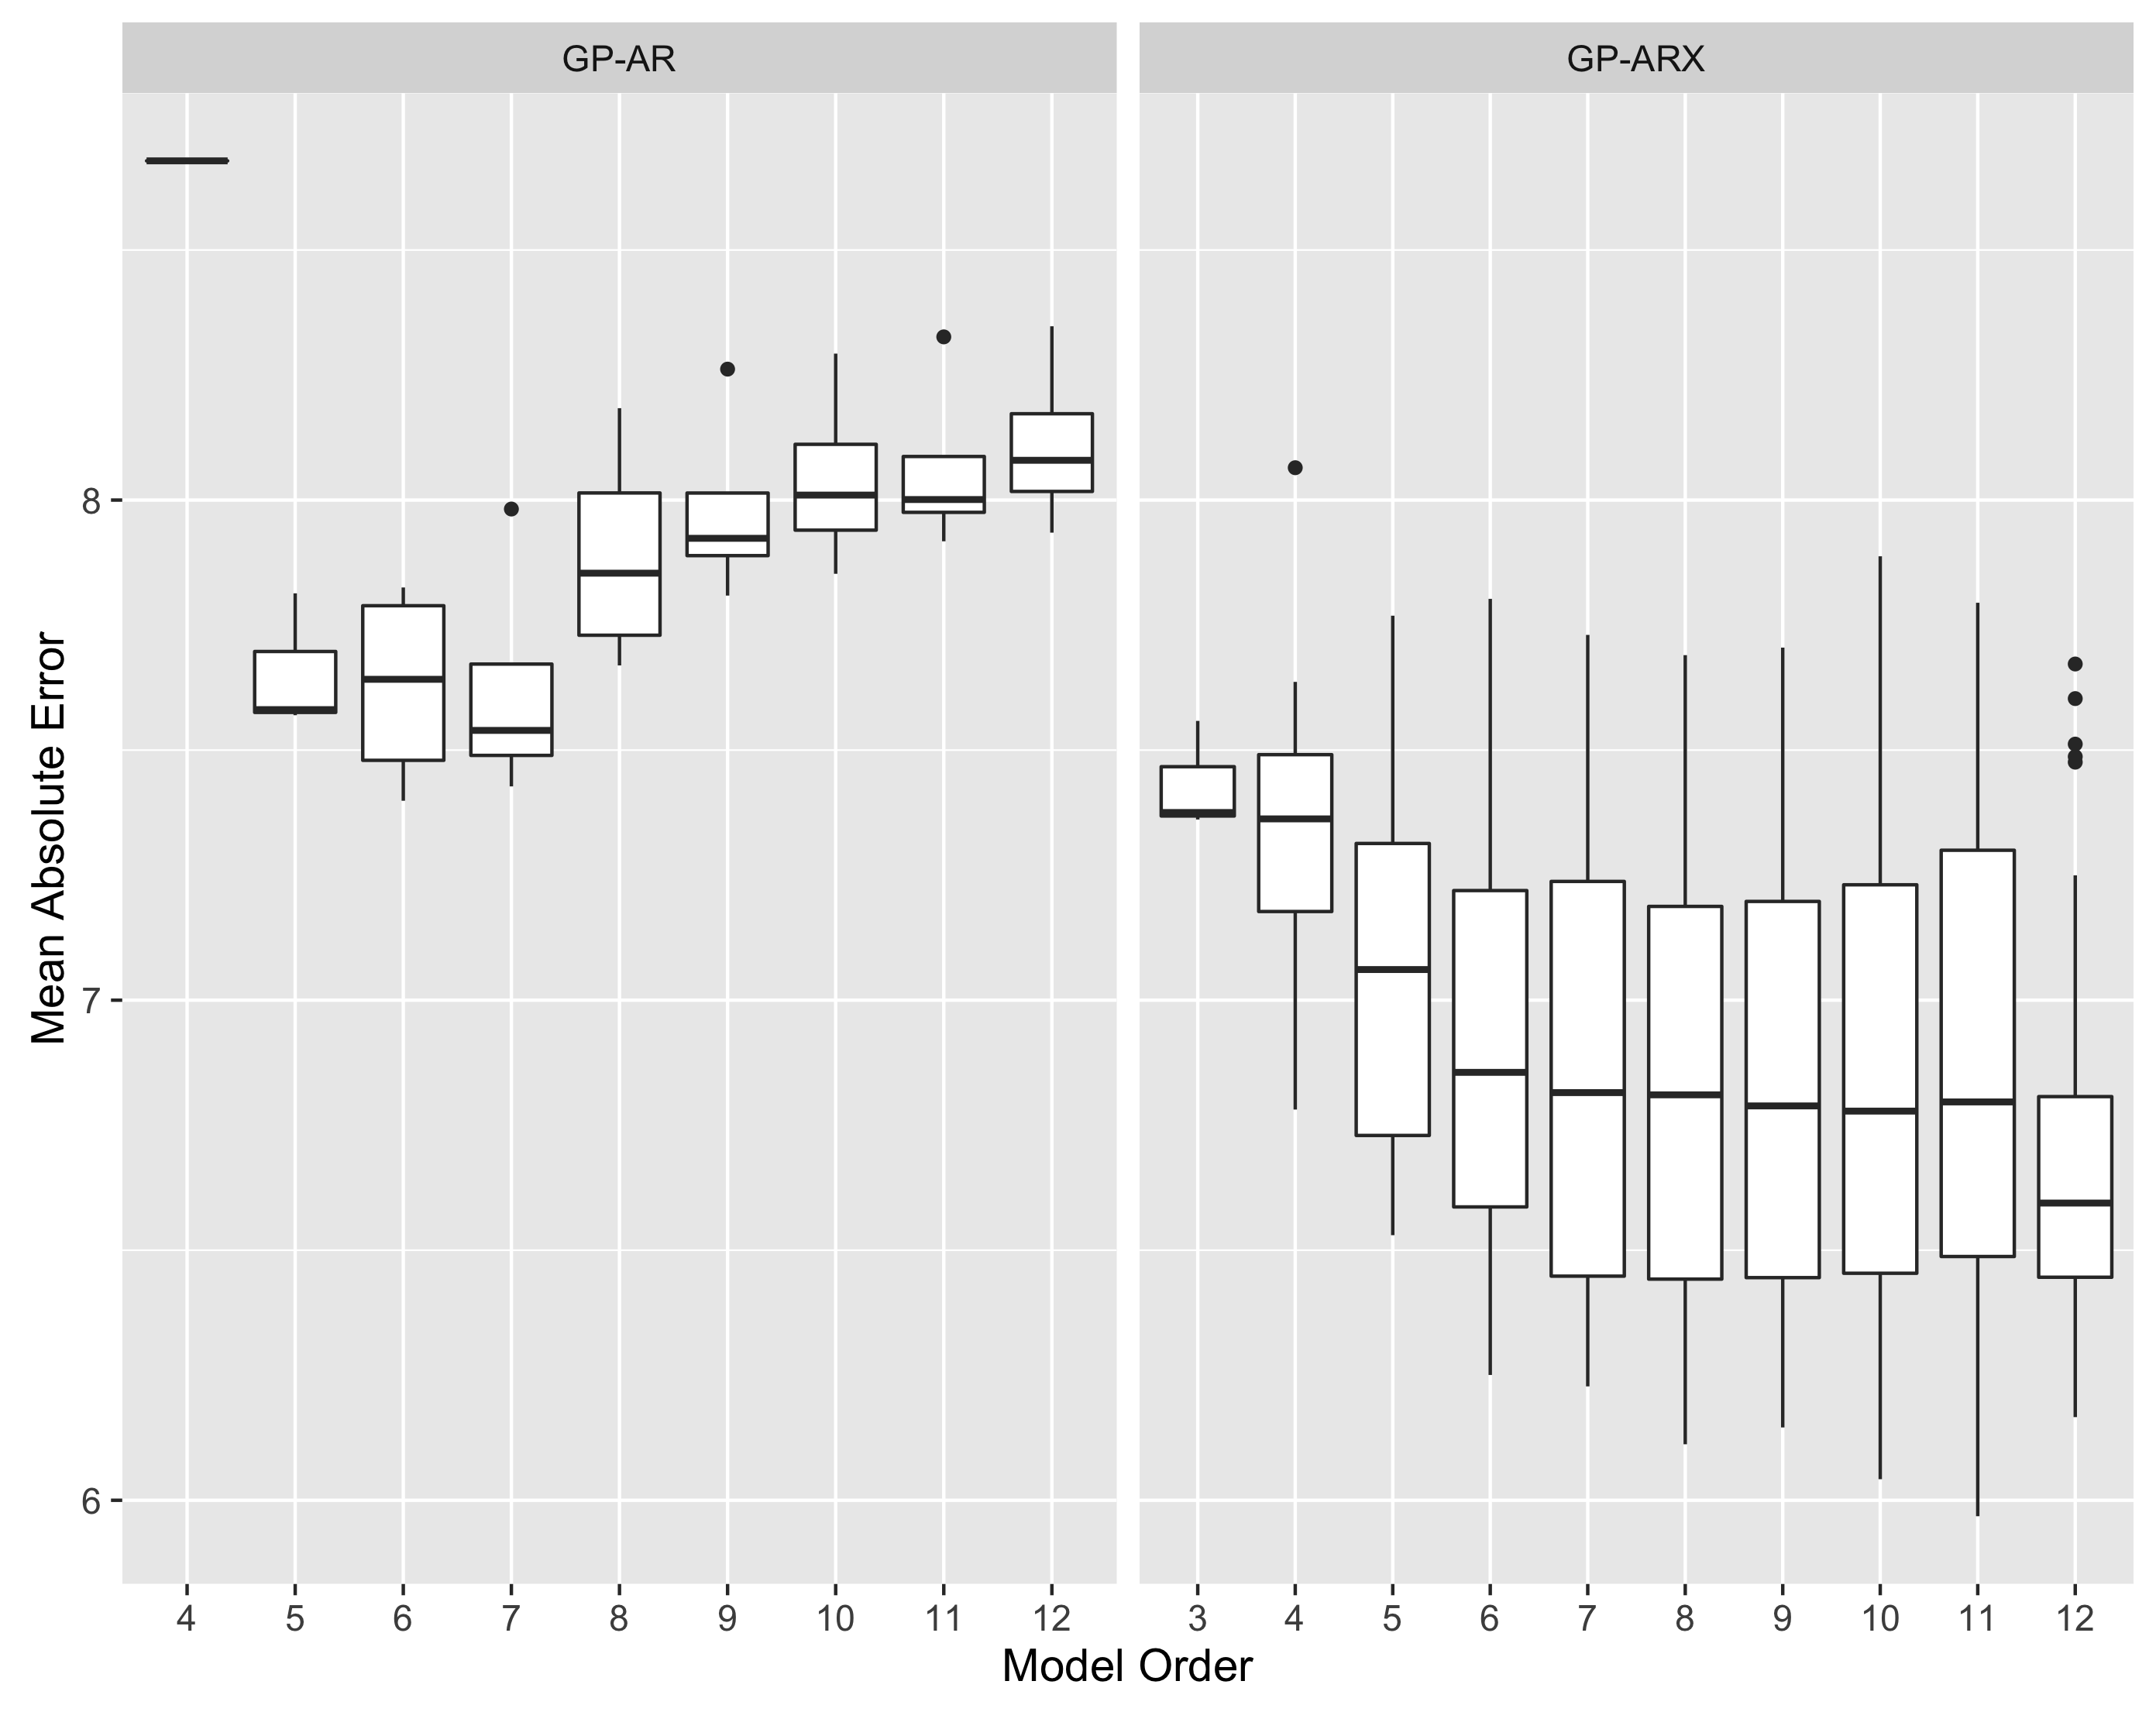
\includegraphics[width=\textwidth]{Compare-mae.png}
\caption{Mean Absolute Error on validation set storms vs model order for GP-AR and GP-ARX. \textbf{Key}: Rectangle borders represent the first and third quartiles, with a horizontal line inside to indicate the median value, outlying points are shown as dots and whiskers indicate the smallest and largest non-outliers}
\label{fig:CompareMae}
\end{figure}

\begin{figure}[h]
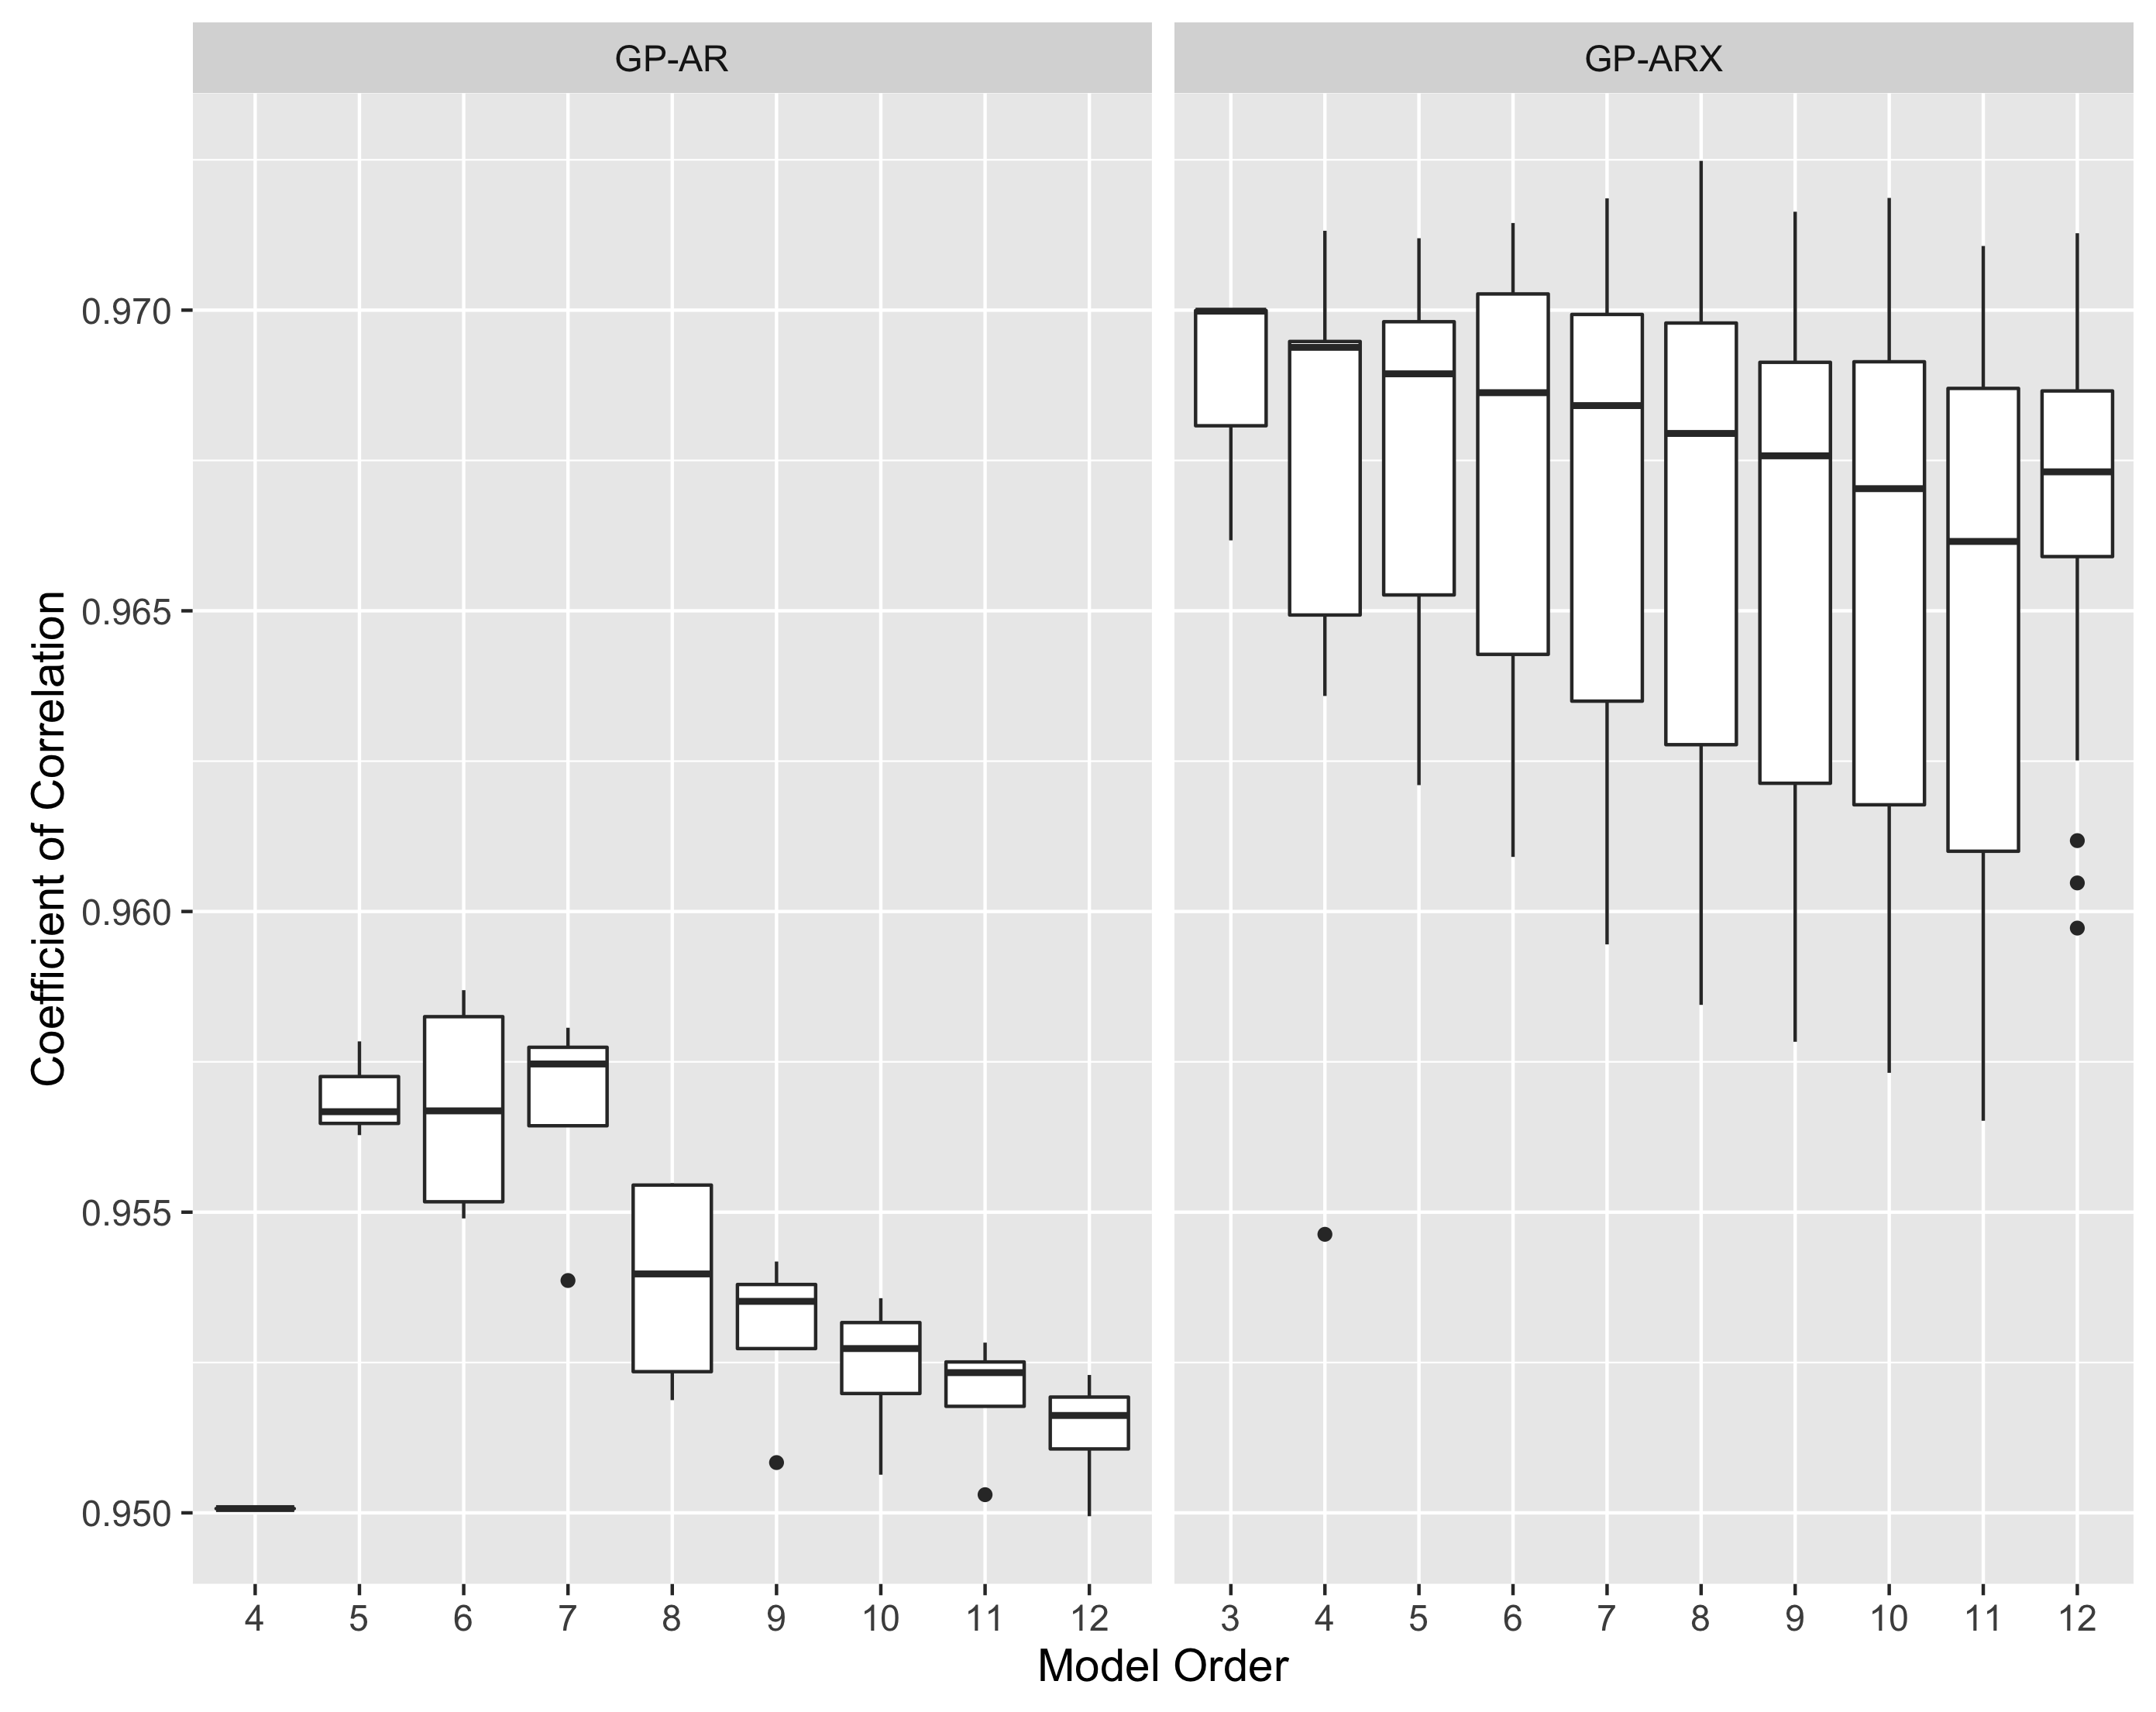
\includegraphics[width=\textwidth]{Compare-cc.png}
\caption{Coefficient of Correlation on validation set storms vs model order for GP-AR and GP-ARX. \textbf{Key}: Rectangle borders represent the first and third quartiles, with a horizontal line inside to indicate the median value, outlying points are shown as dots and whiskers indicate the smallest and largest non-outliers}
\label{fig:CompareCC}
\end{figure}

From the validation results, we can choose the model order which yields the best performance, for GP-AR it is $p_t = 6$ while for GP-ARX it is $p_t = 11$. Further examination of the validation results shows that in the scheme $p_t = 11$ choosing $p = 7, p_v = 1, p_b = 3$ gives superior results.


\subsection*{Comparison of Hyper-parameter Selection Algorithms}
Figures \ref{fig:CompareMaeARX} and \ref{fig:CompareCCARX} break down the results for GP-ARX by the model selection routine used. Apart from the general trend observed in \ref{fig:CompareMae} and \ref{fig:CompareCC}, we also observe that \emph{grid search} and \emph{coupled simulated annealing} give superior performance as compared to gradient based \emph{maximum likelihood}.



\begin{figure}[h]
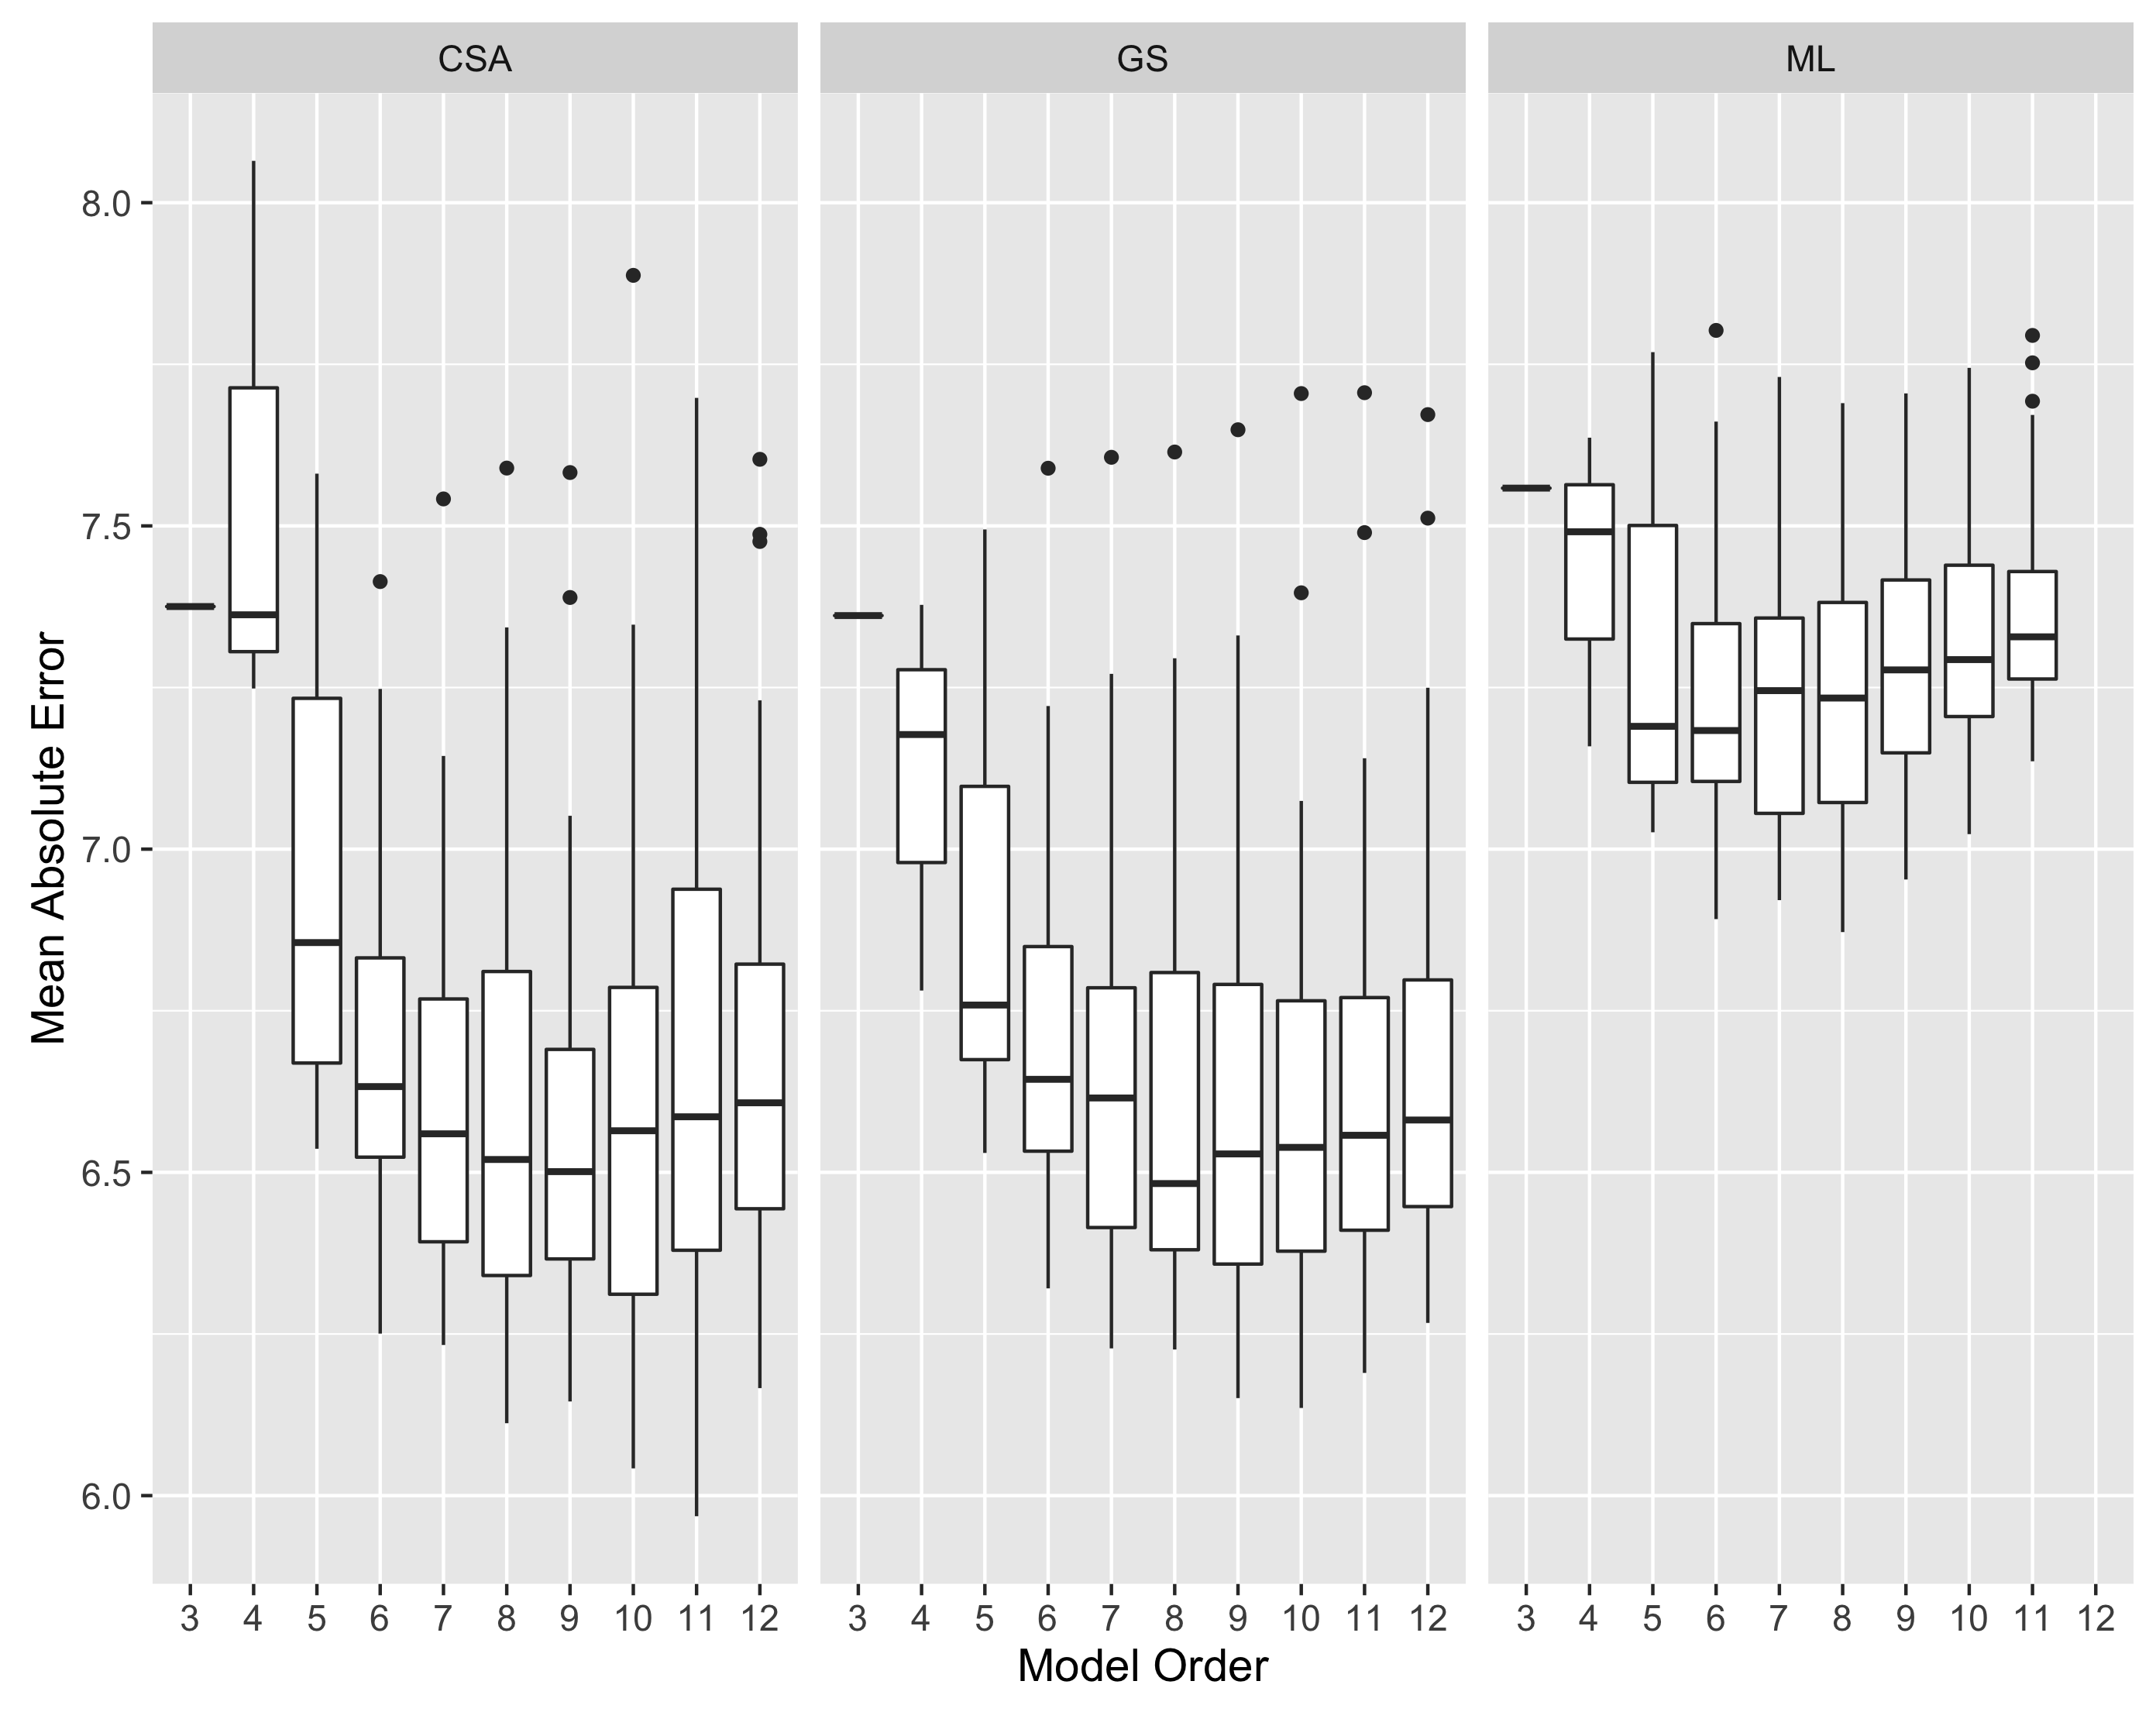
\includegraphics[width=\textwidth]{Compare-mae-arx.png}
\caption{Mean Absolute Error on validation set storms vs model order for GP-AR and GP-ARX for \emph{CSA}, \emph{GS} and \emph{ML} model selection routines. \textbf{Key}: Rectangle borders represent the first and third quartiles, with a horizontal line inside to indicate the median value, outlying points are shown as dots and whiskers indicate the smallest and largest non-outliers}
\label{fig:CompareMaeARX}
\end{figure}

\begin{figure}[h]
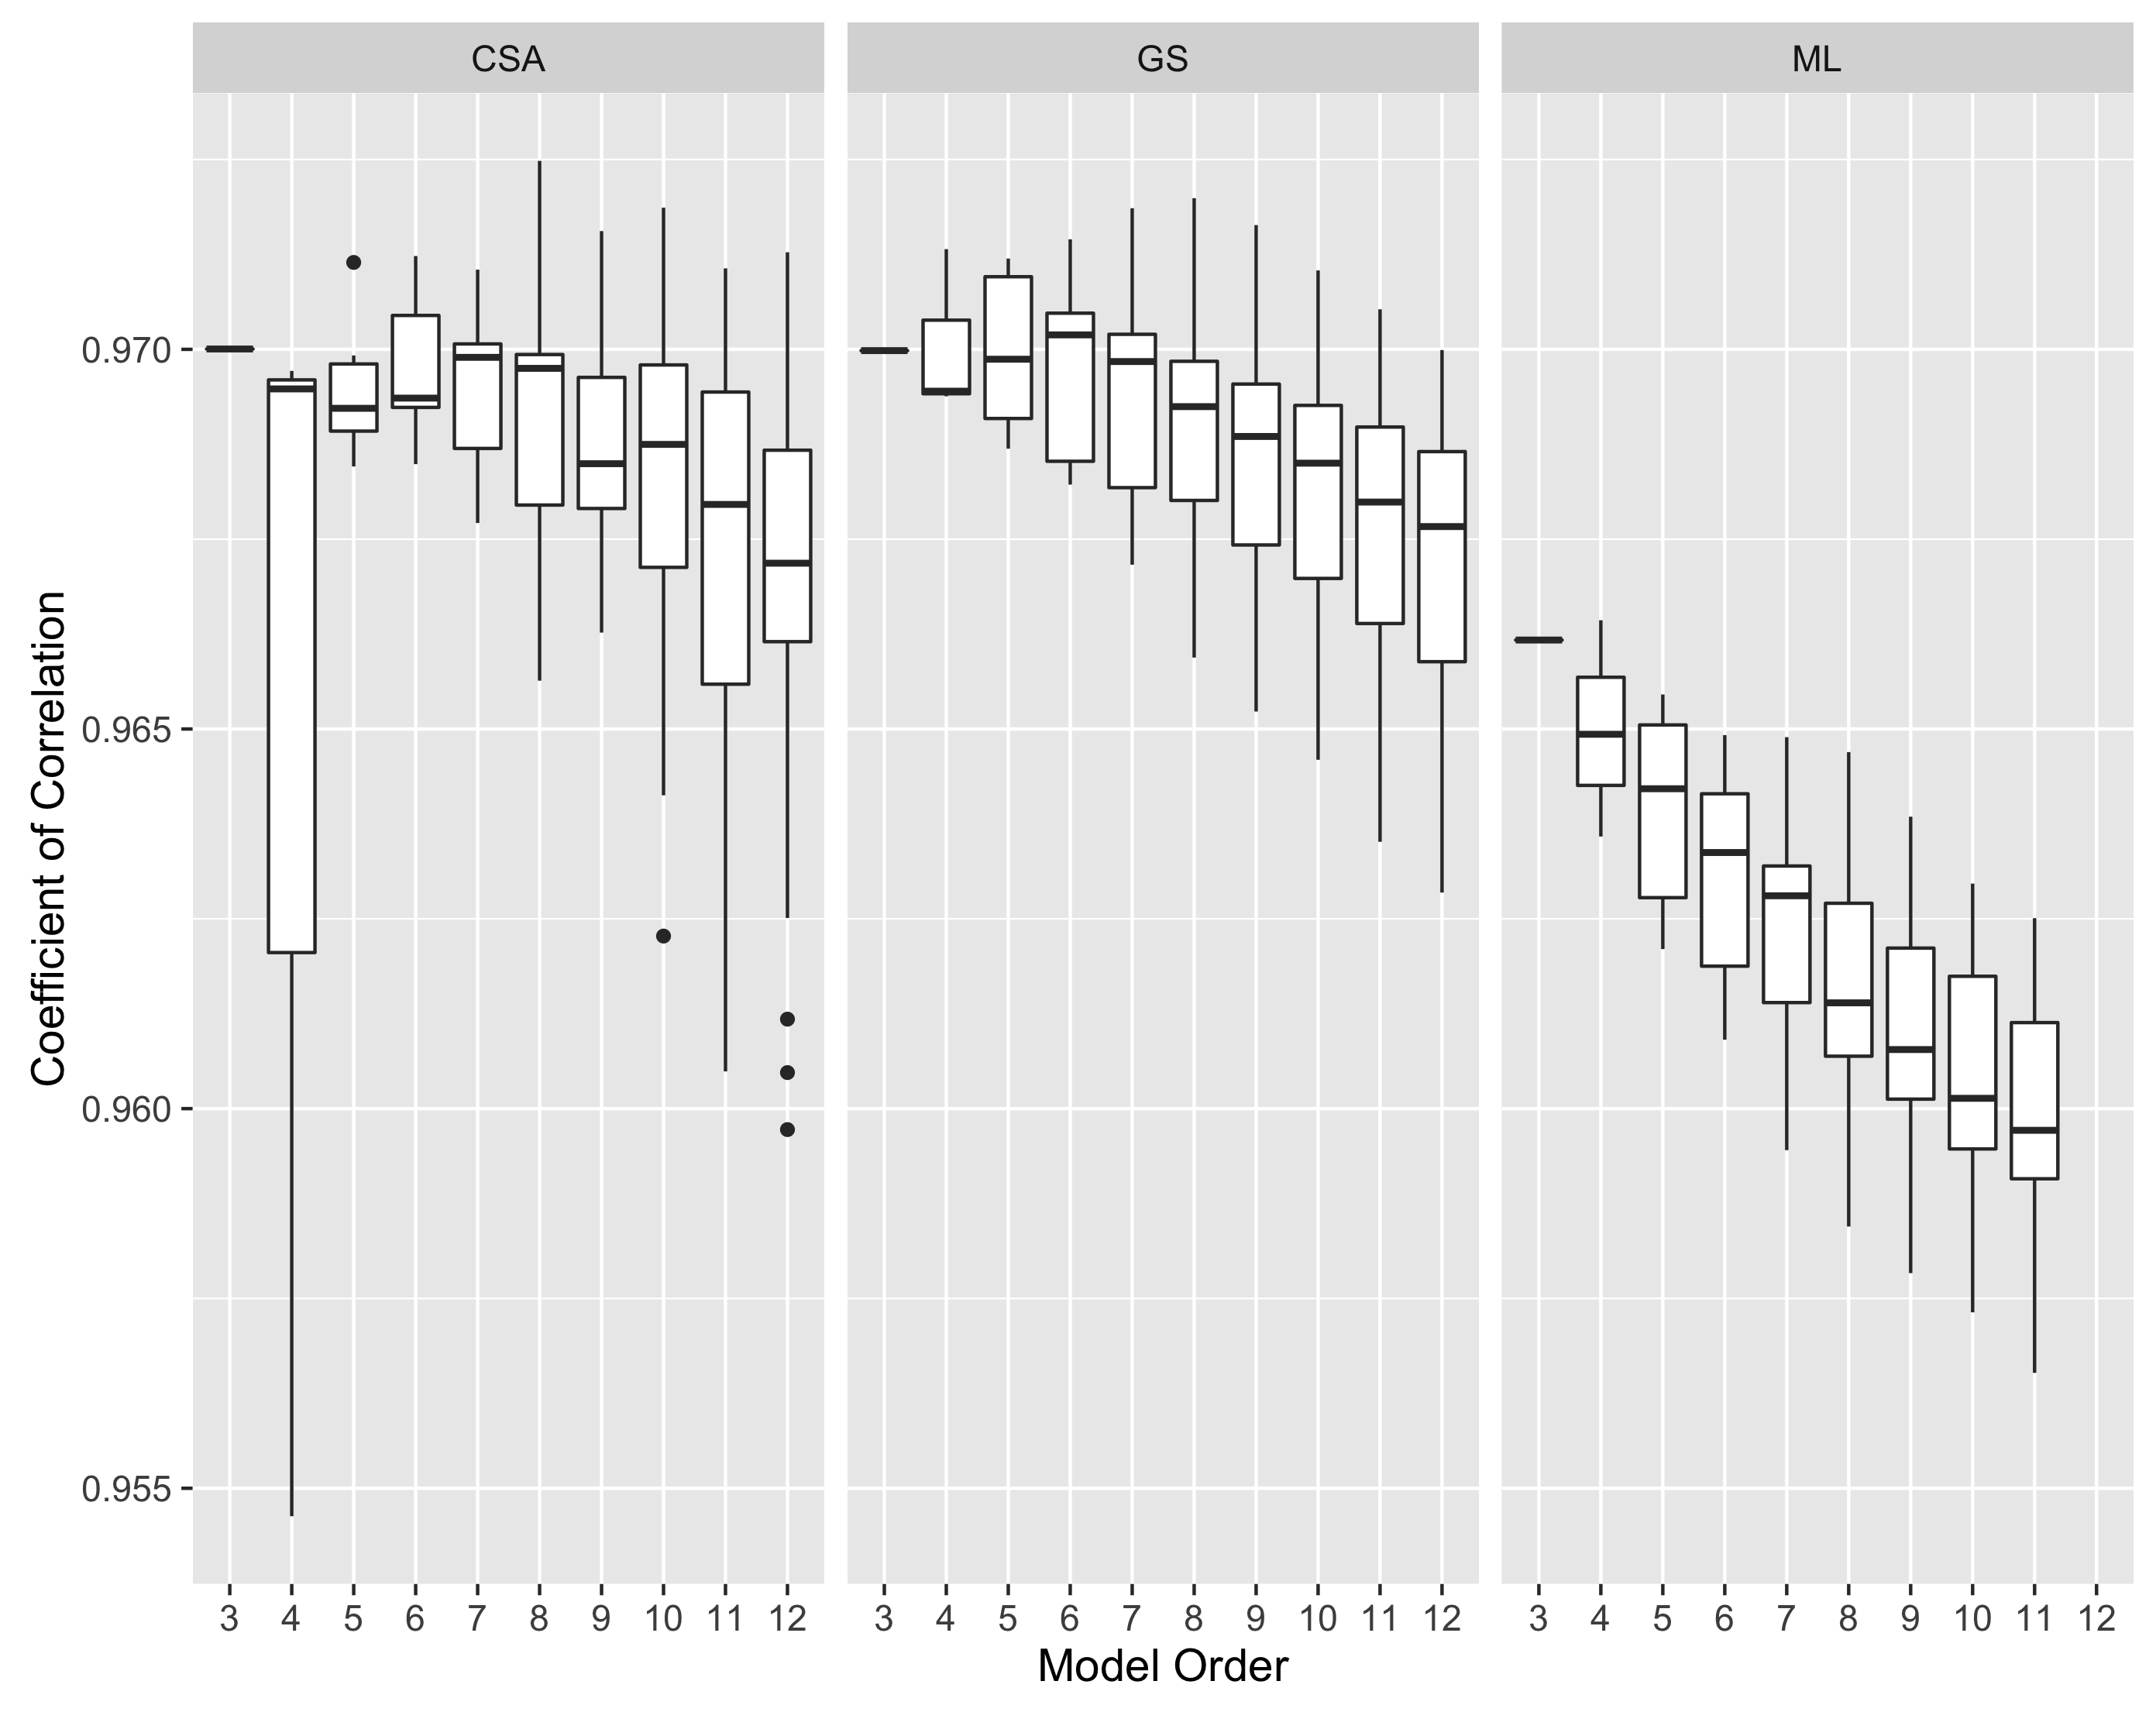
\includegraphics[width=\textwidth]{Compare-cc-arx.png}
\caption{Coefficient of Correlation on validation set storms vs model order for GP-AR and GP-ARX for \emph{CSA}, \emph{GS} and \emph{ML} model selection routines. \textbf{Key}: Rectangle borders represent the first and third quartiles, with a horizontal line inside to indicate the median value, outlying points are shown as dots and whiskers indicate the smallest and largest non-outliers}
\label{fig:CompareCCARX}
\end{figure}

\subsection*{Final Evaluation}

After choosing the best performing GP-AR and GP-ARX models, we calculate their performance on the test set of Table \ref{table:teststorms}. The results of these model evaluations are summarized in Table \ref{table:results}, the GP-AR and GP-ARX models improve upon the performance of the \emph{persistence model}.

\subsection*{Sample Predictions with Error Bars}

Figures \ref{fig:ComparePred1}, \ref{fig:ComparePred2} and \ref{fig:ComparePred3} show OSA predictions of the GP-ARX model with $\pm \sigma$ error bars for three storm events in the time period between 1998 and 2003. The GP-ARX model gives accurate predictions along with plausible error bars around its mean predictions.


\begin{figure}[h]
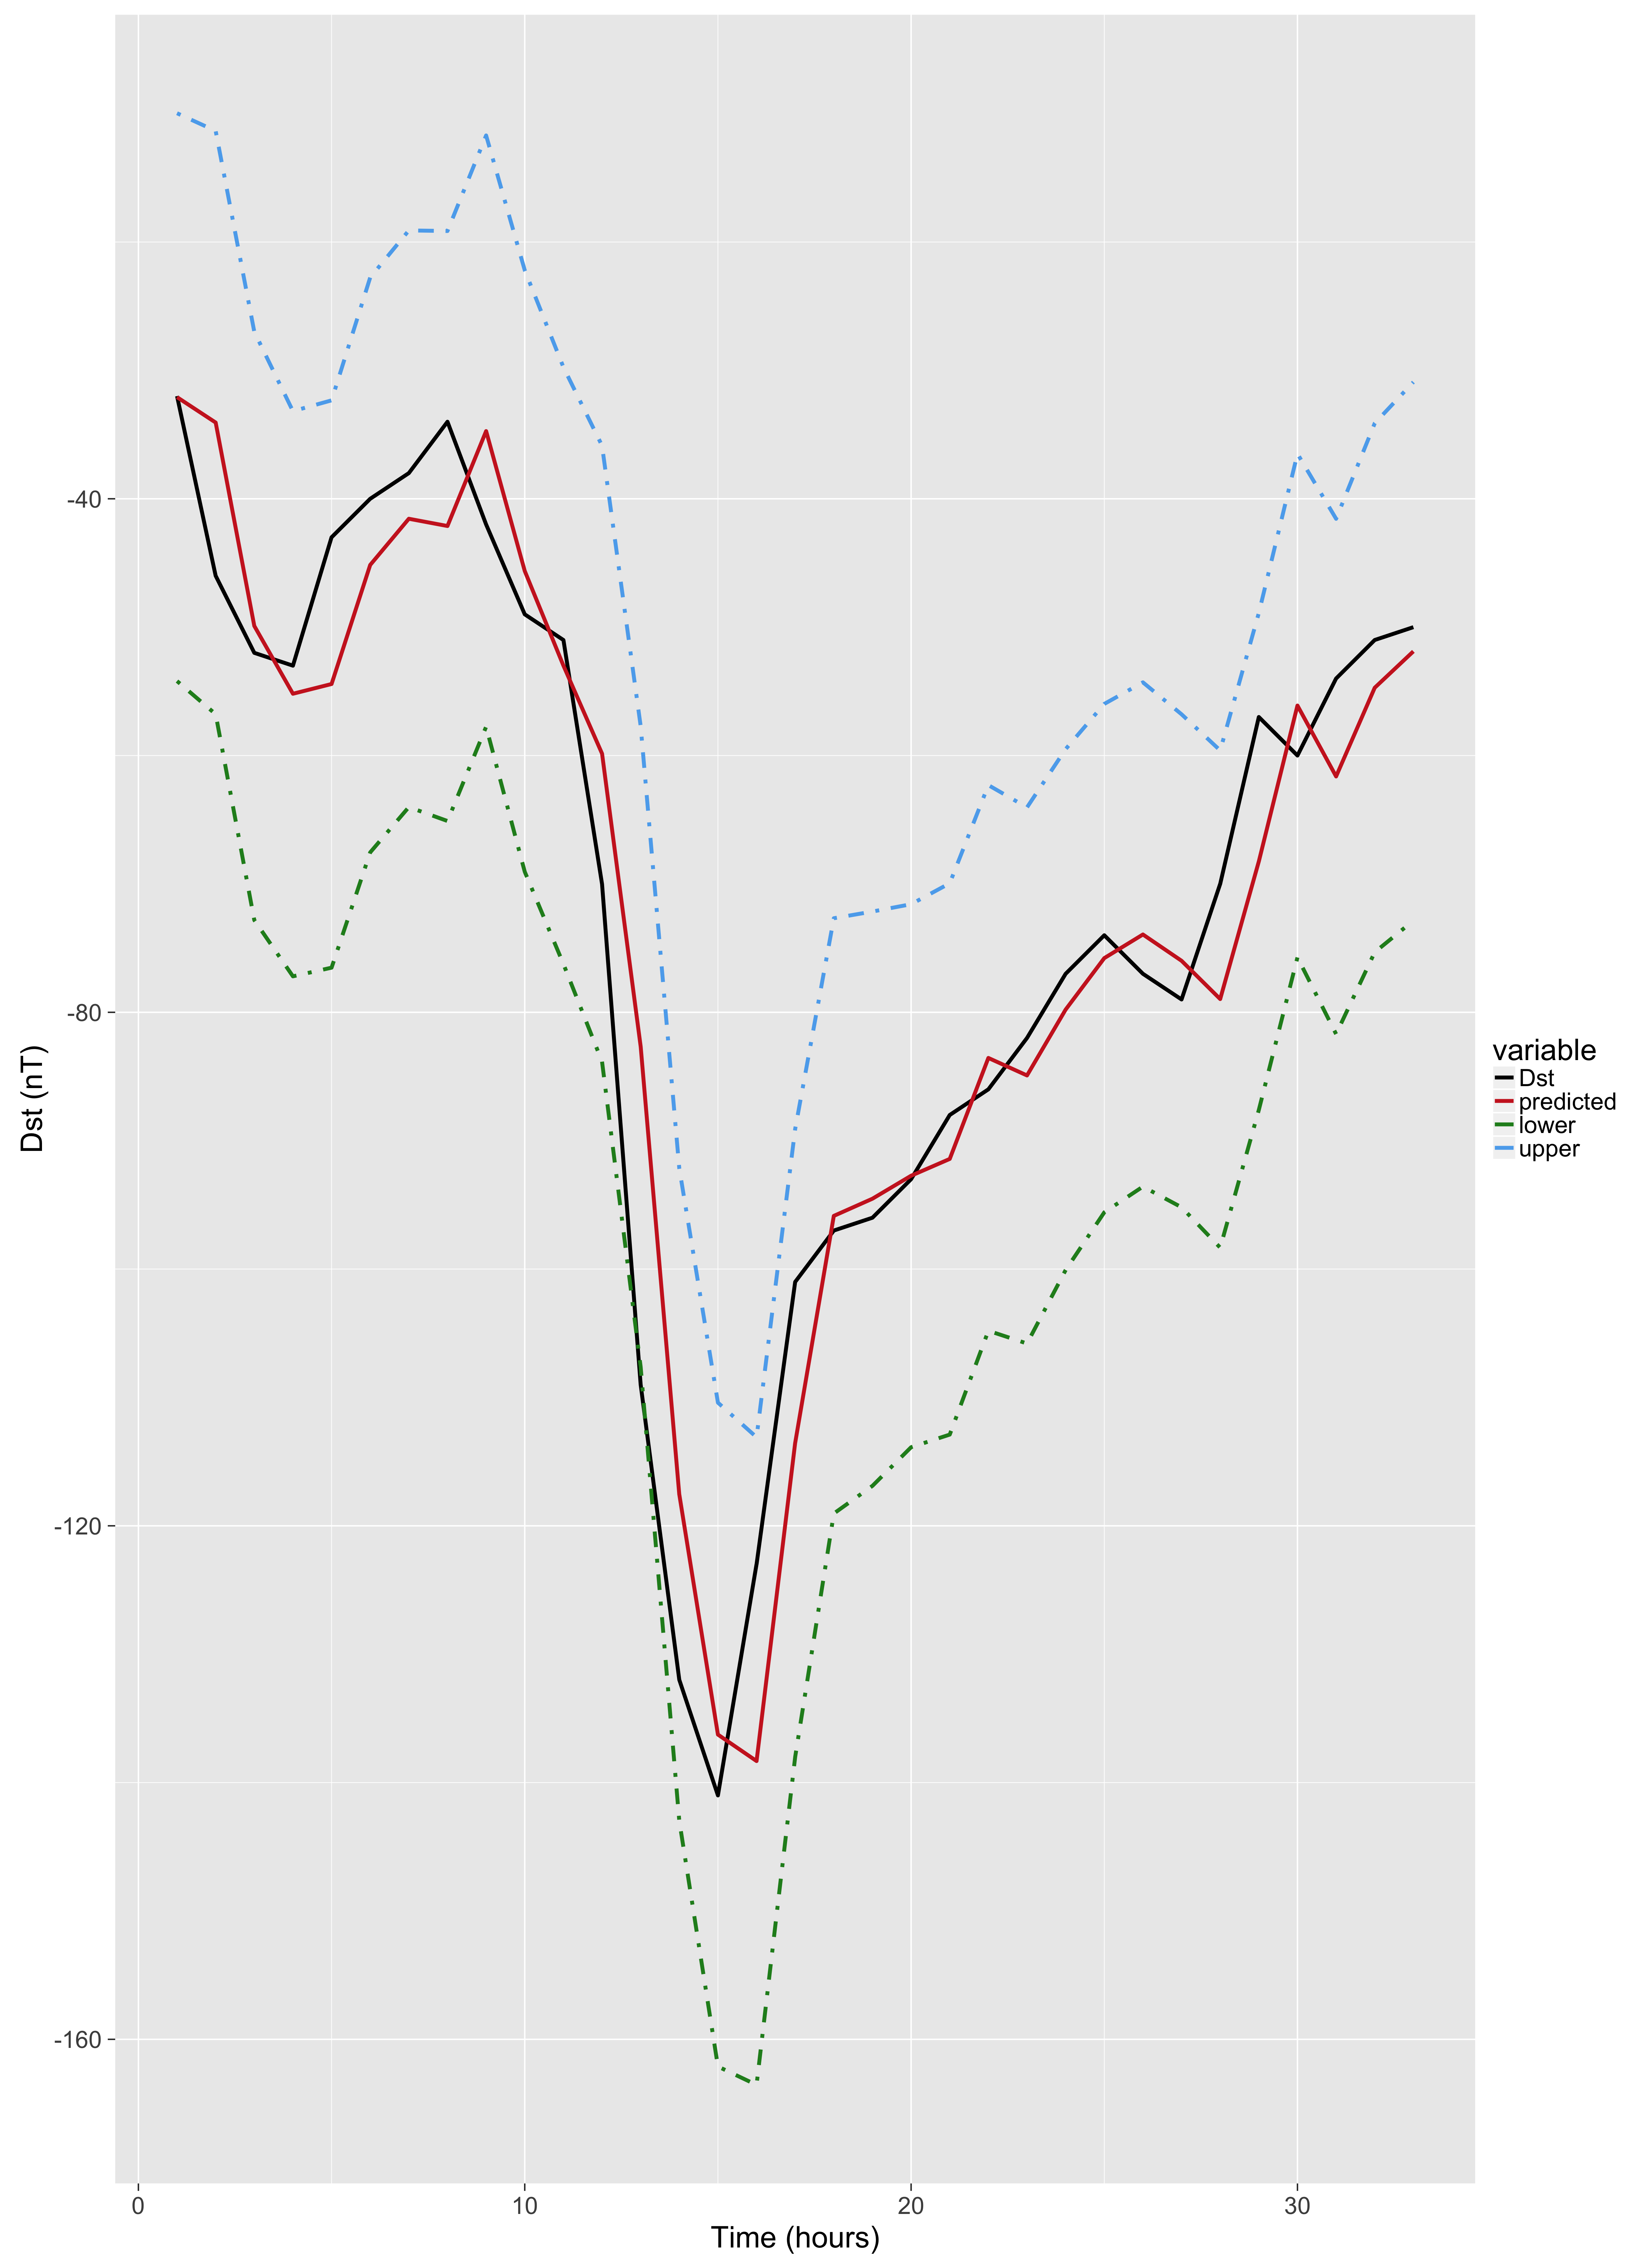
\includegraphics[width=\textwidth]{PredictionsModel1/PredErrBars_Storm43.png}
\caption{OSA Predictions with $\pm \sigma$ error bars for event: 2003/06/17 to 2003/06/19}
\label{fig:ComparePred1}
\end{figure}


\begin{figure}[h]
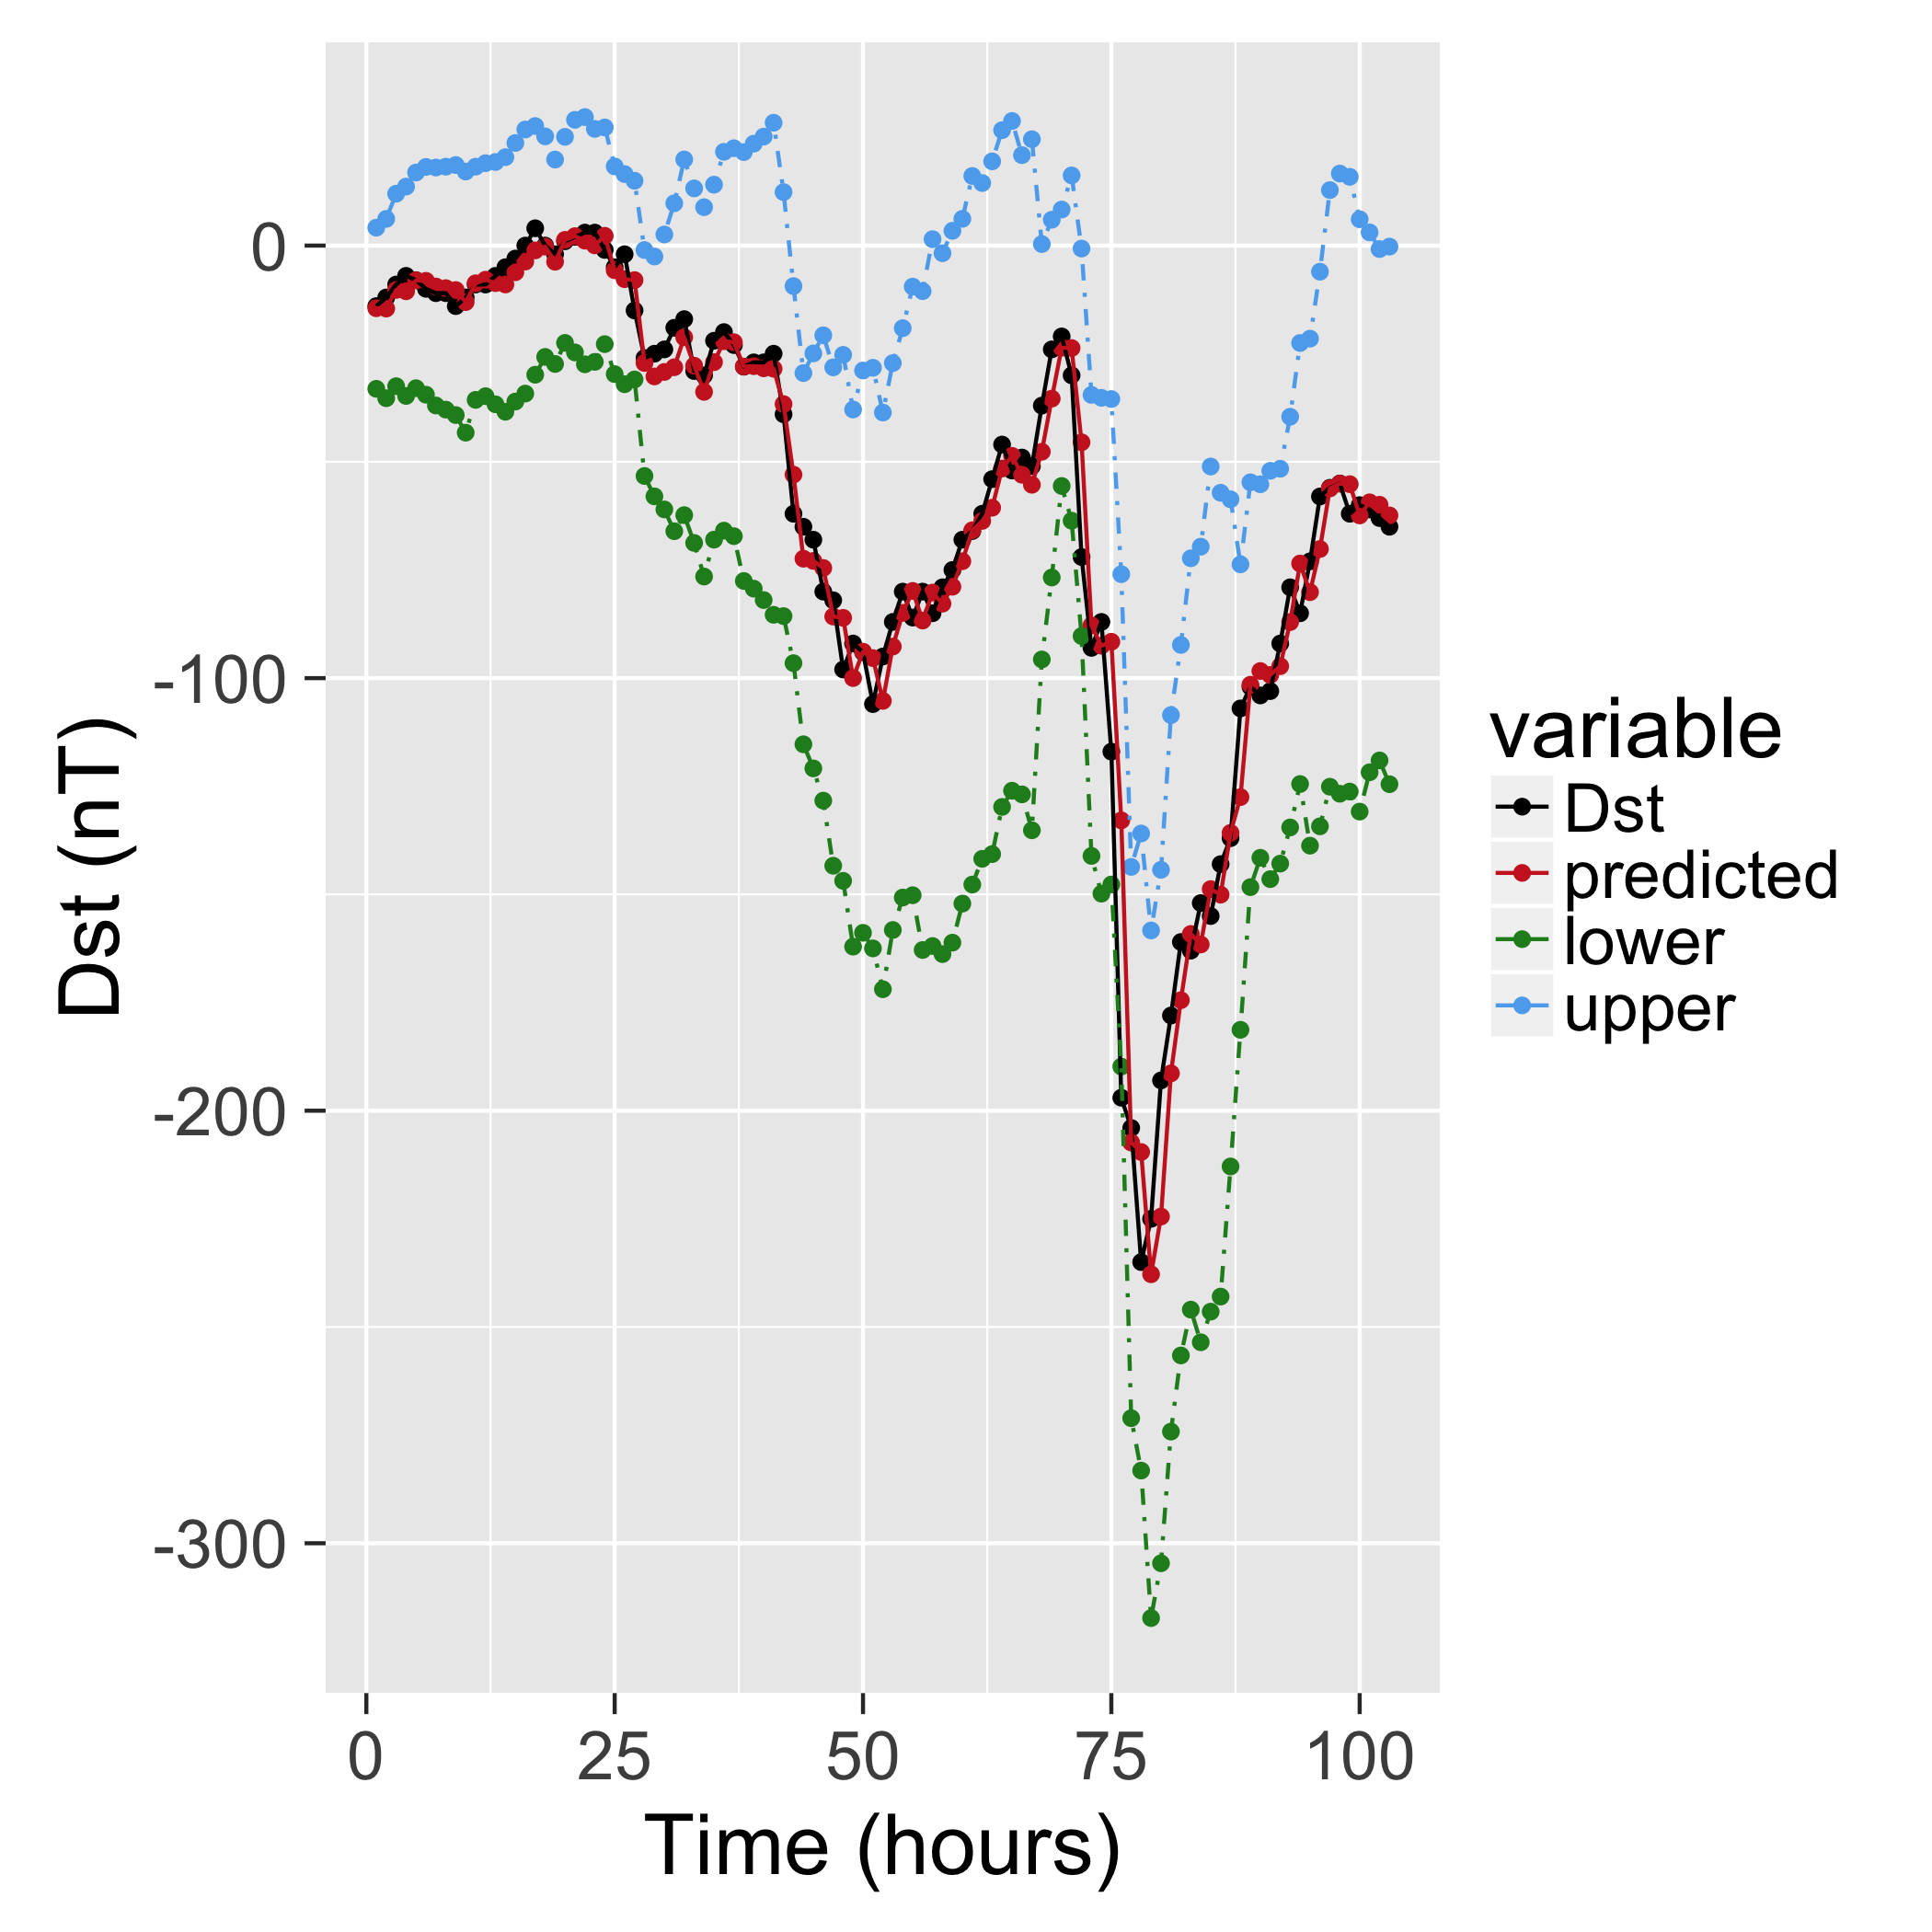
\includegraphics[width=\textwidth]{PredictionsModel1/PredErrBars_Storm16.png}
\caption{OSA Predictions with $\pm \sigma$ error bars for event: 2012/03/08 to 2012/03/10}
\label{fig:ComparePred2}
\end{figure}

\begin{figure}[h]
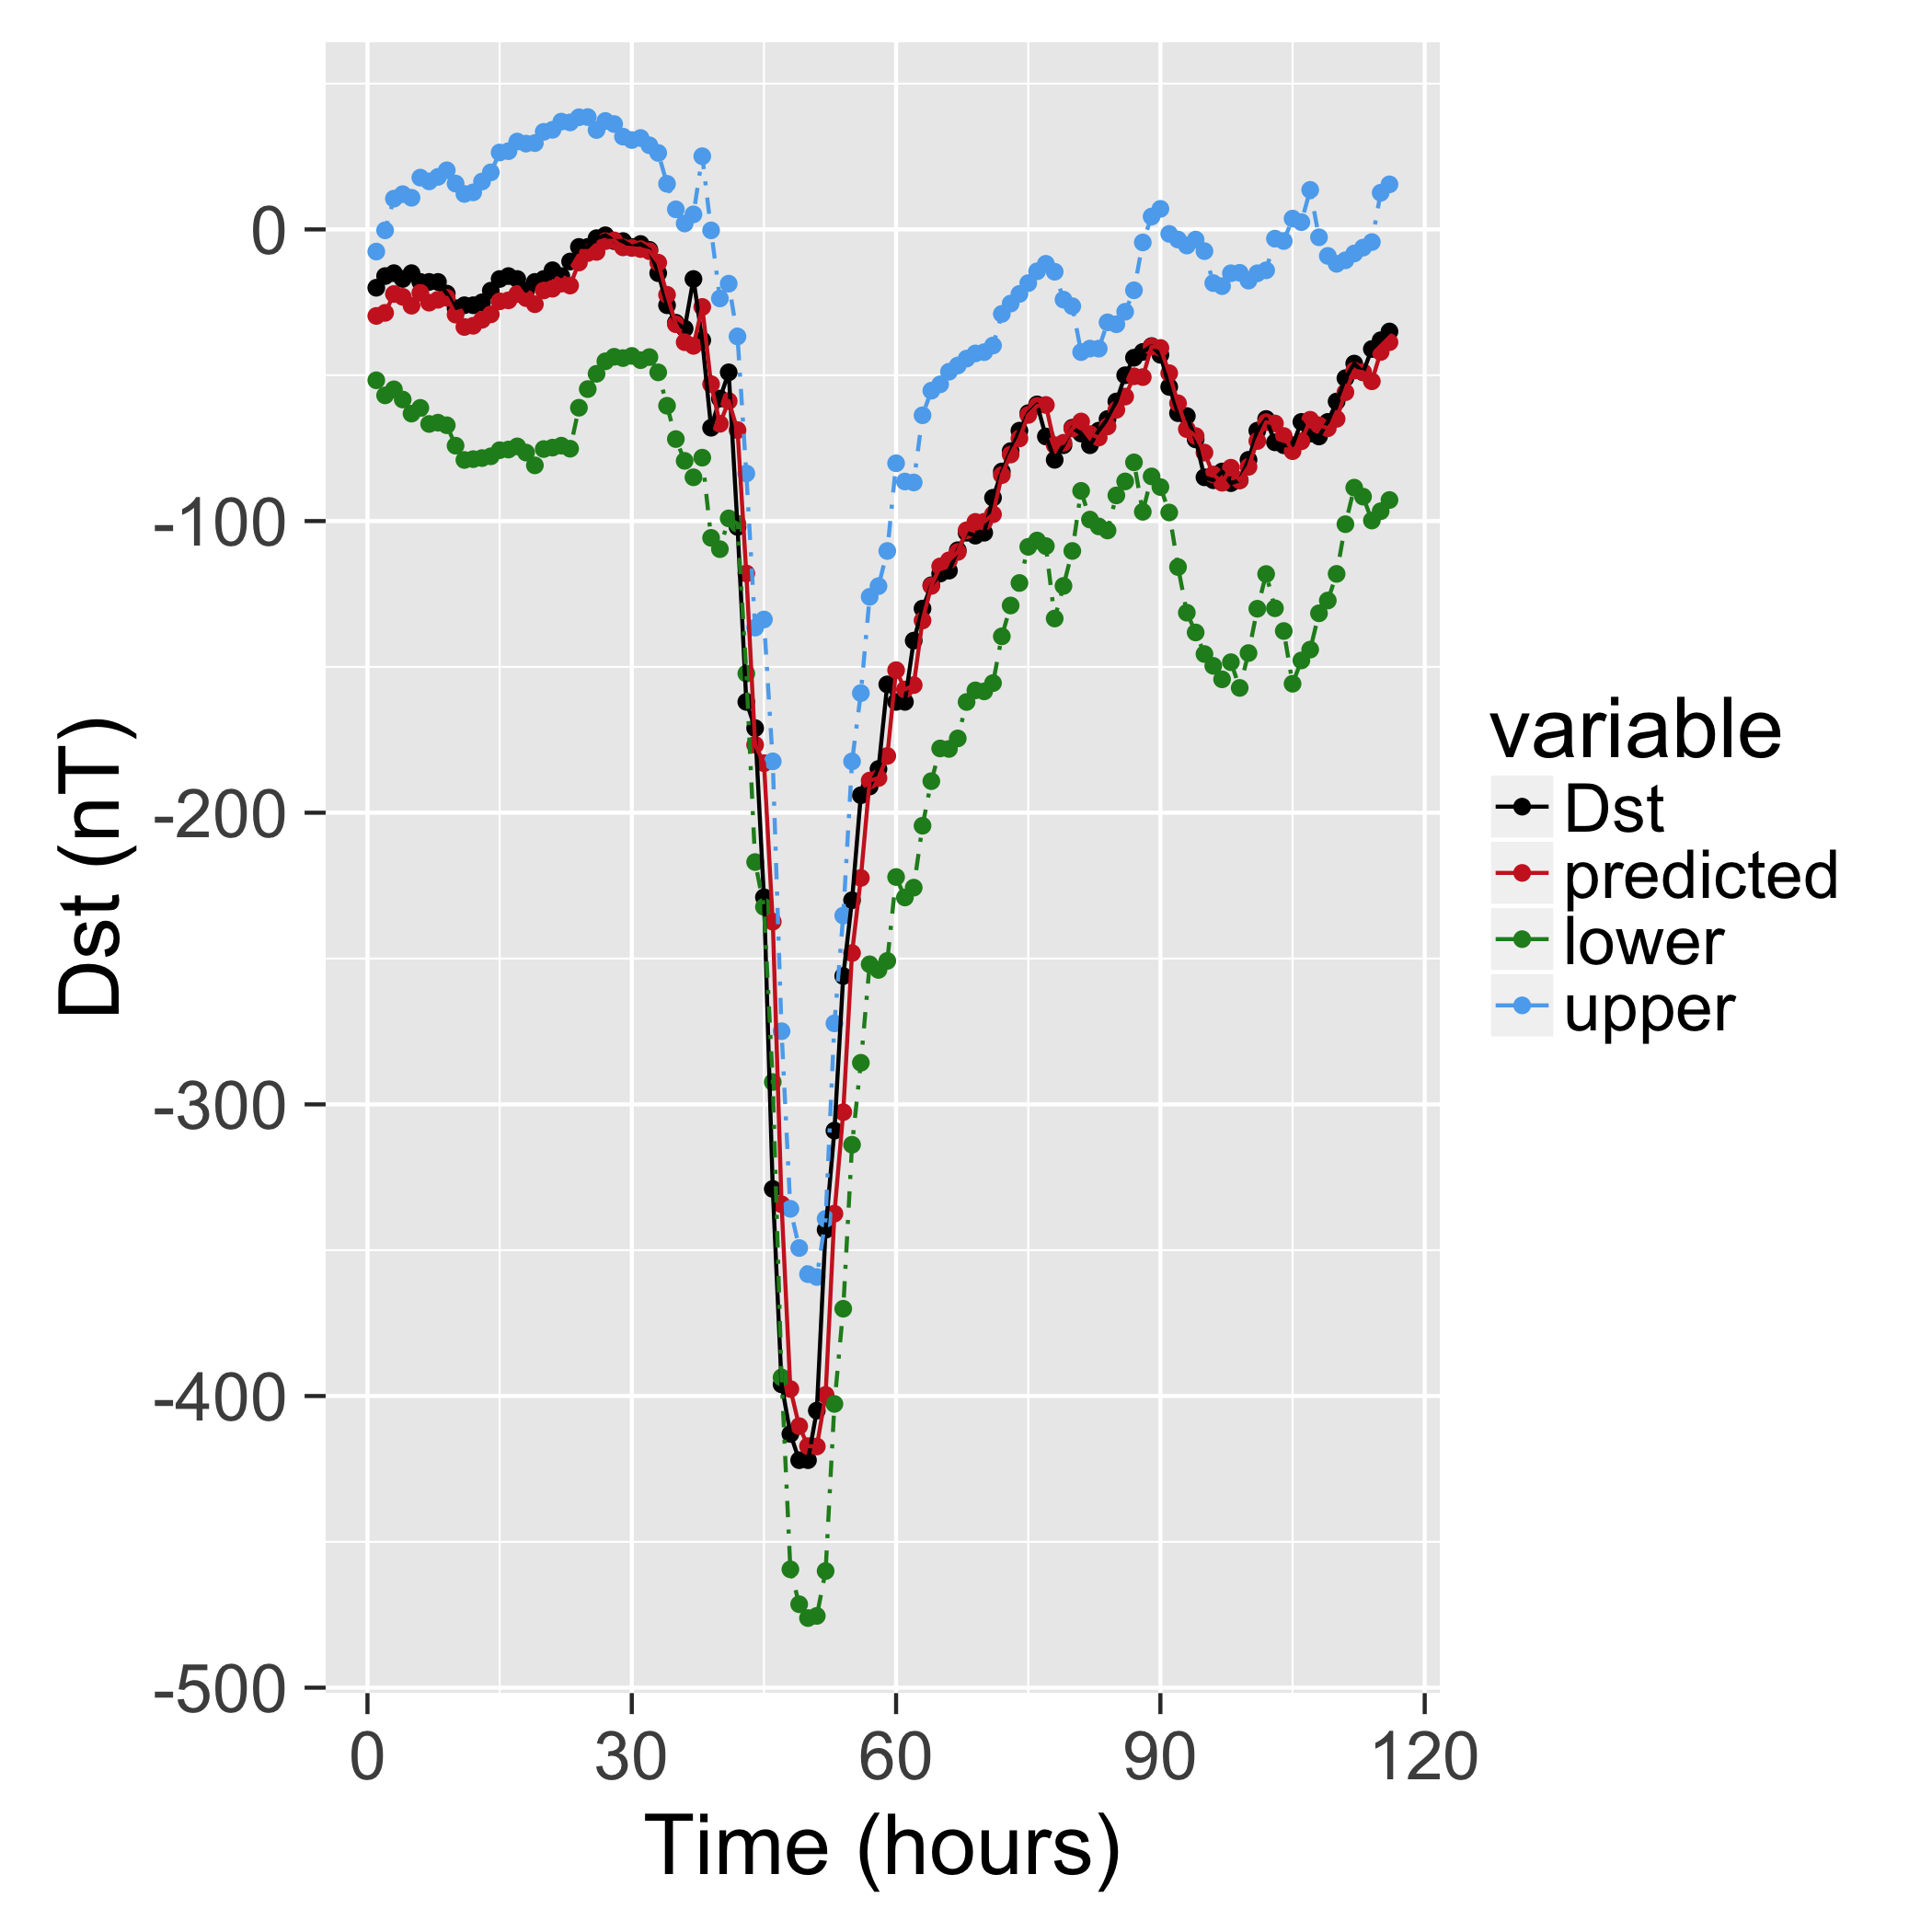
\includegraphics[width=\textwidth]{PredictionsModel1/PredErrBars_Storm46.png}
\caption{OSA Predictions with $\pm \sigma$ error bars for event: 2003/11/20 to 2003/11/22}
\label{fig:ComparePred3}
\end{figure}




\begin{table}[h]
\centering
\caption{Settings of model selection procedures}
\begin{tabular}{l c c c}
\hline
Procedure & Grid Size & Step & Max Iterations \\
\hline
Grid Search & 10 & 0.2 & NA \\
Coupled Simulated Annealing & 4 & 0.2 & 30 \\
Maximum likelihood & NA & 0.2 & 150\\
\end{tabular}
\label{table:modelselection}
\end{table}



\begin{table}[h]
\centering
\caption{Storm events used for model selection of GP-AR and GP-ARX}
\label{table:validationstorms}
\begin{tabular}{llllll}
\hline
Event Id & Start Date & Start Hour & End Date & End Hour & min. Dst \\ \hline
1 & 1995/03/26 & 0500 & 1995/03/26 & 2300 & −107 \\
2 & 1995/04/07 & 1300 & 1995/04/09 & 0900 & −149 \\
3 & 1995/09/27 & 0100 & 1995/09/28 & 0400 & −108 \\
4 & 1995/10/18 & 1300 & 1995/10/19 & 1400 & −127 \\
5 & 1996/10/22 & 2200 & 1996/10/23 & 1100 & −105 \\
6 & 1997/04/21 & 1000 & 1997/04/22 & 0900 & −107 \\
7 & 1997/05/15 & 0300 & 1997/05/16 & 0000 & −115 \\
8 & 1997/10/10 & 1800 & 1997/10/11 & 1900 & −130 \\
9 & 1997/11/07 & 0000 & 1997/11/07 & 1800 & −110 \\
10 & 1997/11/22 & 2100 & 1997/11/24 & 0400 & −108 \\
11 & 2005/06/12 & 1700 & 2005/06/13 & 1900 & −106 \\
12 & 2005/08/31 & 1200 & 2005/09/01 & 1200 & −122 \\
13 & 2006/12/14 & 2100 & 2006/12/16 & 0300 & −162 \\
14 & 2011/09/26 & 1400 & 2011/09/27 & 1200 & −101 \\
15 & 2011/10/24 & 2000 & 2011/10/25 & 1400 & −132 \\
16 & 2012/03/08 & 1200 & 2012/03/10 & 1600 & −131 \\
17 & 2012/04/23 & 1100 & 2012/04/24 & 1300 & −108 \\
18 & 2012/07/15 & 0100 & 2012/07/16 & 2300 & −127 \\
19 & 2012/09/30 & 1300 & 2012/10/01 & 1800 & −119 \\
20 & 2012/10/08 & 0200 & 2012/10/09 & 1700 & −105 \\
21 & 2012/11/13 & 1800 & 2012/11/14 & 1800 & −108 \\
22 & 2013/03/17 & 0700 & 2013/03/18 & 1000 & −132 \\
23 & 2013/05/31 & 1800 & 2013/06/01 & 2000 & −119 \\
24 & 2014/02/18 & 1500 & 2014/02/19 & 1600 & −112
\end{tabular}
\end{table}


\begin{table}[h]
\fontsize{6}{7.5}\selectfont
\centering
\caption{Storm events used to evaluate GP-AR and GP-ARX models}
\label{table:teststorms}
\begin{tabular}{cccccc}
\hline
Event Id & Start Date & Start Time & End Date & End Time & min. Dst \\ \hline
1 & 1998/02/17 & 1200 & 1998/02/18 & 1000 & -100 \\
2 & 1998/03/10 & 1100 & 1998/03/11 & 1800 & -116 \\
3 & 1998/05/04 & 0200 & 1998/05/05 & 0200 & -205 \\
4 & 1998/08/26 & 1000 & 1998/08/29 & 0700 & -155 \\
5 & 1998/09/25 & 0100 & 1998/09/26 & 0000 & -207 \\
6 & 1998/10/19 & 0500 & 1998/10/20 & 0800 & -112 \\
7 & 1998/11/09 & 0300 & 1998/11/10 & 1600 & -142 \\
8 & 1998/11/13 & 0000 & 1998/11/15 & 0400 & -131 \\
9 & 1999/01/13 & 1600 & 1999/01/14 & 2000 & -112 \\
10 & 1999/02/18 & 0300 & 1999/02/19 & 2100 & -123 \\
11 & 1999/09/22 & 2000 & 1999/09/23 & 2300 & -173 \\
12 & 1999/10/22 & 0000 & 1999/10/23 & 1400 & -237 \\
13 & 2000/02/12 & 0500 & 2000/02/13 & 1500 & -133 \\
14 & 2000/04/06 & 1700 & 2000/04/08 & 0900 & -288 \\
15 & 2000/05/24 & 0100 & 2000/05/25 & 2000 & -147 \\
16 & 2000/08/10 & 2000 & 2000/08/11 & 1800 & -106 \\
17 & 2000/08/12 & 0200 & 2000/08/13 & 1700 & -235 \\
18 & 2000/10/13 & 0200 & 2000/10/14 & 2300 & -107 \\
19 & 2000/10/28 & 2000 & 2000/10/29 & 2000 & -127 \\
20 & 2000/11/06 & 1300 & 2000/11/07 & 1800 & -159 \\
21 & 2000/11/28 & 1800 & 2000/11/29 & 2300 & -119 \\
22 & 2001/03/19 & 1500 & 2001/03/21 & 2300 & -149 \\
23 & 2001/03/31 & 0400 & 2001/04/01 & 2100 & -387 \\
24 & 2001/04/11 & 1600 & 2001/04/13 & 0700 & -271 \\
25 & 2001/04/18 & 0100 & 2001/04/18 & 1300 & -114 \\
26 & 2001/04/22 & 0200 & 2001/04/23 & 1500 & -102 \\
27 & 2001/08/17 & 1600 & 2001/08/18 & 1600 & -105 \\
28 & 2001/09/30 & 2300 & 2001/10/02 & 0000 & -148 \\
29 & 2001/10/21 & 1700 & 2001/10/24 & 1100 & -187 \\
30 & 2001/10/28 & 0300 & 2001/10/29 & 2200 & -157 \\
31 & 2002/03/23 & 1400 & 2002/03/25 & 0500 & -100 \\
32 & 2002/04/17 & 1100 & 2002/04/19 & 0200 & -127 \\
33 & 2002/04/19 & 0900 & 2002/04/21 & 0600 & -149 \\
34 & 2002/05/11 & 1000 & 2002/05/12 & 1600 & -110 \\
35 & 2002/05/23 & 1200 & 2002/05/24 & 2300 & -109 \\
36 & 2002/08/01 & 2300 & 2002/08/02 & 0900 & -102 \\
37 & 2002/09/04 & 0100 & 2002/09/05 & 0000 & -109 \\
38 & 2002/09/07 & 1400 & 2002/09/08 & 2000 & -181 \\
39 & 2002/10/01 & 0600 & 2002/10/03 & 0800 & -176 \\
40 & 2002/10/03 & 1000 & 2002/10/04 & 1800 & -146 \\
41 & 2002/11/20 & 1600 & 2002/11/22 & 0600 & -128 \\
42 & 2003/05/29 & 2000 & 2003/05/30 & 1000 & -144 \\
43 & 2003/06/17 & 1900 & 2003/06/19 & 0300 & -141 \\
44 & 2003/07/11 & 1500 & 2003/07/12 & 1600 & -105 \\
45 & 2003/08/17 & 1800 & 2003/08/19 & 1100 & -148 \\
46 & 2003/11/20 & 1200 & 2003/11/22 & 0000 & -422 \\
47 & 2004/01/22 & 0300 & 2004/01/24 & 0000 & -149 \\
48 & 2004/02/11 & 1000 & 2004/02/12 & 0000 & -105 \\
49 & 2004/04/03 & 1400 & 2004/04/04 & 0800 & -112 \\
50 & 2004/07/22 & 2000 & 2004/07/23 & 2000 & -101 \\
51 & 2004/07/24 & 2100 & 2004/07/26 & 1700 & -148 \\
52 & 2004/07/26 & 2200 & 2004/07/30 & 0500 & -197 \\
53 & 2004/08/30 & 0500 & 2004/08/31 & 2100 & -126 \\
54 & 2004/11/07 & 2100 & 2004/11/08 & 2100 & -373 \\
55 & 2004/11/09 & 1100 & 2004/11/11 & 0900 & -289 \\
56 & 2004/11/11 & 2200 & 2004/11/13 & 1300 & -109 \\
57 & 2005/01/21 & 1800 & 2005/01/23 & 0500 & -105 \\
58 & 2005/05/07 & 2000 & 2005/05/09 & 1000 & -127 \\
59 & 2005/05/29 & 2200 & 2005/05/31 & 0800 & -138 \\
60 & 2005/06/12 & 1700 & 2005/06/13 & 1900 & -106 \\
61 & 2005/08/31 & 1200 & 2005/09/01 & 1200 & -131 \\
62 & 2006/04/13 & 2000 & 2006/04/14 & 2300 & -111 \\
63 & 2006/12/14 & 2100 & 2006/12/16 & 0300 & -147 \\ \hline
\end{tabular}%
\end{table}



\begin{table}[h]
\centering
\caption{Evaluation results for models on storm events listed in table \ref{table:teststorms}}
\label{table:results}
\begin{tabular}{l c c c}
\hline
Model & Mean Absolute Error & Root Mean Square Error & Coefficient of Correlation\\ \hline
GP-ARX & 7.252 & 11.93 & 0.972\\
GP-AR & 8.37 & 14.04 & 0.963\\
Persistence & 9.182 & 14.94 & 0.957\\
\end{tabular}
\end{table}


\clearpage 

\bibliography{references}

\end{document}